
\section{Création de Personnage}
\lettrine{L}{e} c\oe{}ur des jeux de rôle réside dans la possibilité de créer, améliorer et faire évoluer son propre personnage. Voilà comment ça fonctionne dans {\jedifont \doctitle}. 

\subsection{Les Attributs}
Chaque personnage commence le jeu avec d4 dans chaque Attribut et dispose de 5pt pour les améliorer. Améliorer l’un d’entre eux d’un type de dé (par exemple, de d4 à d6) coûte 1 point avec une limite : vous ne pouvez aller au-delà du d12.

\subsection{Compétences}
Les Compétences représentent les aptitudes apprises comme le Tir, le Combat, les connaissances professionnelles ou scientifiques et ainsi de suite. Elles sont générales et englobent tous les aspects qui leur sont reliés. Par exemple Tir englobe les fusils, les arcs, les lance-roquettes et toutes les armes à distance. Vous disposez de 15 points à répartir entre vos Compétences. Chaque dé de Compétence coûte 1 point (en commençant à d4) tant qu’il est inférieur ou égal à l’Attribut dont il dépend (noté entre parenthèses près du nom de la Compétence). Chaque dé de Compétence supérieur à l’Attribut dont il dépend coûte 2 points. De même que pour les Attributs, aucune Compétence ne peut dépasser d12.

\subsection{Atouts \& Handicaps}
Faire naître un héros digne de ce nom ne se limite pas à lui faire grimper ses attributs et ses compétences. Ce qui fait la singularité d’un héros et qui le rend fun à jouer c’est ses Atouts et ses Handicaps. De la blonde très séduisante au Vieux maître Jedi, vous prendrez toujours plus de plaisir à jouer un personnage unique dans ses détails que le jeune humain sans problème que vous êtes tout les jours.

Vous pouvez choisir jusqu’à 1 Handicap Majeur et 2 Handicaps Mineurs. Un Handicap Majeur donne 2 points et un Handicap Mineur 1 point.

Pour 2 points vous pouvez :
\begin{rebelist}
    \item Augmenter un Attribut d’un type de dé (vous pouvez le faire avant de prendre vos Compétences).
    \item Choisir un Atout.
\end{rebelist}

Pour 1 point vous pouvez :
\begin{rebelist}
    \item Gagner un point de Compétence.
    \item Doubler vos fonds de départ (si vous débutez avec 500\crg vous obtenez 500\crg de plus).
\end{rebelist}

\subsection{Races Jouables}
Vous pouvez choisir pour votre personnage n’importe quelle race disponible dans L’univers de Star Wars. L’orientation de chaque race est donnée à titre indicatif, chaque race possède des exceptions parmi ses héros.

\subsubsection{Humain}
\begin{samepage}
	\begin{flushright}
		\begin{tabular}{|l|r|}
			\textbf{Type} 			& Humanoïde \\
		   	\textbf{Planète} 		& Terre \\
		   	\textbf{Langage} 		& Basic \\
		   	\textbf{Orientation} 	& Neutre \\
		\end{tabular}
	\end{flushright}

	\vspace{-6\baselineskip}
	\includegraphics[width=5cm]{img/personnages/races/humain.png} 
\end{samepage}

Cette race comprend aussi bien les humains au sens strict (qu’ils soient originaires de Coruscant, de Correlia, de Kuat, de Naboo\ldots) que les humanoïdes dont les caractéristiques physiques, intellectuelles, sociales et culturelles sont suffisamment proches de celles des humains pour qu’il soit possible de les assimiler en termes de jeu.

\begin{description}[align=left]
\item [Adaptabilité] 	%CAP +2
	Les humains sont une race pleine de ressources, ils s’adaptent rapidement à toutes sorte de difficultés ou environnements.\\
	\textit{Atout Novice gratuit}
\end{description}
\newpage
\subsubsection{Barabel}
\begin{samepage}
    \begin{flushright}	
        \begin{tabular}{|l|r|}
            \textbf{Type}        & Reptile \\
            \textbf{Planète}     & Barab I \\
            \textbf{Langage}     & Barabel \\
            \textbf{Orientation} & Obscur \\
        \end{tabular}
    \end{flushright}

	\vspace{-5\baselineskip}
	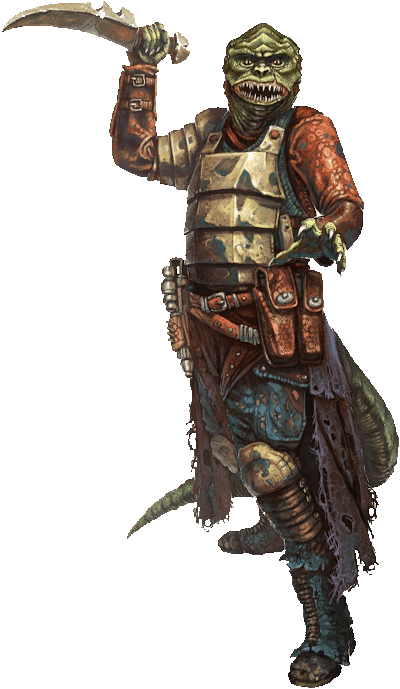
\includegraphics[width=5cm]{img/personnages/races/barabel.png}
\end{samepage}

Originaire de Barab I, les Barabels sont restés une race relativement primitive et isolée. Les Barabels vivent en clans dans un société principalement matriarcale. Ils sont fascinés par la guerre, la violence et les armes. Les Barabels ne sont pas profondément cruels, mais ils restent agressifs de nature. En raison des nombreux rituels précédent les négociations, la diplomatie avec les Barabels est un exercice compliqué.

Le Barabel adulte est un reptile bipède dont la taille dépasse toujours les deux mètres. Sa dentition est formée d’une multitude de dents en forme d’aiguilles qui peuvent atteindre jusqu’à cinq centimètres de long et ses mains sont équipées de griffes puissantes.

\begin{description}[align=left]
\item [Enfance difficile] 	% CAP +1 +1
		De par l’environnement hostile de leur planète natale, les Barabels possèdent une résistance accrue à la chaleur et aux radiations.\\
		\textit{+4 en Résistance à la chaleur}\\
		\textit{+4 en Résistance aux radiations}
\item [\OE{il} Ophidien] 	% CAP +1
		Les yeux ophidiens du Barabel lui permettent de capter la plupart des ondes lumineuses allant du jaune à l’infrarouge, mais il confond facilement les couleurs tirant dans les bleus et violets.\\
		\textit{Infravision}
\item [Arme naturelle]		% CAP +1
		Les mains des Barabels sont équipés de puissante griffes.\\
		\textit{For + d6 de dégâts}
\item [Balayage]			% CAP +2
		Les Barabels utilise leur appendice caudal d’instinct dans les combats.\\
		\textit{+ Atout Balayage}
\item [Primitif]			% CAP -3
		Les Barabels sont une race encore primitive.\\
		\textit{Int <= d6}
\item [Dur d’oreille]		% CAP -1
		Les Barabels en tant que reptilien ne possède pas d’oreille, ils entendent par vibrations.\\
		\textit{Dur d’oreille (Mineur)}
\end{description}
\newpage
\subsubsection{Besalisk}
\vspace{-2\baselineskip}
\begin{flushright}	
    \begin{tabular}{|l|r|}
        \textbf{Type} & Reptile \\
        \textbf{Planete} & Ojom \\
        \textbf{Langage} & Basic \\
        \textbf{Orientation} & Neutre\\
    \end{tabular}
\end{flushright}
\vspace{-3\baselineskip}
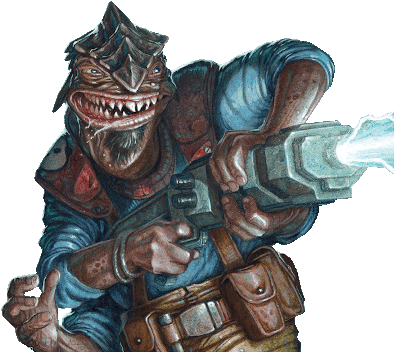
\includegraphics[width=8cm]{img/personnages/races/besalisk.png}
 
Les Besalisks sont trapus et possèdent des bras très imposants, ils sont également entourés de petits plumes autour de la crête osseuse. Reptiles bipèdes, Originaires d’une planète glacière ils sont naturellement insensibles au froid, d’excellents grimpeurs et nageurs.

\begin{description}[align=left]
\item [A bras le corps]         % +2 
    Les mâles ont 4 bras, les deux supérieurs pour l’utilisation d’ustensiles et les deux inférieurs pour agripper.\\
    \textit{Action supplémentaire gratuite}

\item [Pas frileux]             % +1 +1 -1
    Les Besalisks ont développé des facultés physiques particulières pour supporter les conditions climatiques rudes de leur planète. En effet, Ojom est une planète couverte d’un océan froid où de gigantesques icebergs se déplacent.\\
    \textit{+4 Résistance au froid}\\
    \textit{-4 Résistance à la chaleur}\\
    \textit{Natation d6}

\item [Bricoleur]               % +2
    Bien qu’au niveau technologique leur race n’ait pas apporté quelque chose de concret à la galaxie, ils assimilent sans trop de difficulté le fonctionnement de nombreux appareils\\
    \textit{Atout Bidouilleur}

\item [Dette de Liberté]        % -2
    Ojom, la planète natale des Besalisk s’est trouvé épargné par l’empire grâce à des faveurs qui rend la plupart des Besalisks redevable à une race. Le background du perso détermine la race.\\
    \textit{Handicap Code d’honneur}

\item [Loyal]                   % -1
    Les Besalisks sont une race d’êtres sociables et surtout loyaux. Ils donneraient leur vie pour leurs coéquipiers.\\
    \textit{Handicap Loyal}
\end{description}
\subsubsection{Bothan}

\begin{samepage}
	\includegraphics[width=5cm]{img/personnages/races/bothan.png}
	\vspace{-16\baselineskip}
	\begin{flushright}
		\begin{tabular}{|l|r|}
			\textbf{Type} 			& Félin \\
		   	\textbf{Planète} 		& Bothawui \\
		   	\textbf{Langage} 		& Bothese \\
		   	\textbf{Orientation} 	& Lumineux \\
		\end{tabular}
	\end{flushright}
    \vspace{11\baselineskip}
\end{samepage}

Les Bothans sont des humanoïdes trapus, dont le corps est recouvert d’une épaisse fourrure pouvant varier du blanc-cassé à brun très foncé.
Le peuple bothan est originaire de la planète Bothawui, un monde cosmopolite épargné des troubles de la Guerre Civile Galactique en raison de la neutralité officielle du gouvernement bothan. Plusieurs colonies ont également été construites sur des planètes proches, telles que Kothlis, qui est désormais le siège d’une importante communauté. Toutes ces colonies forment l’Espace Bothan.\\
La structure sociale des Bothans est constituée de clans familiaux, dont le nom est inclus dans le nom de chaque Bothan, à la suite d’une apostrophe.

\begin{description}[align=left]
\item [Agilité du Félin] 			% CAP +2
		Les Bothans possède la grâce de leurs ancêtres félins.\\
		\textit{Commence avec d6 Agi}

\item [Service de renseignement] 	% CAP +1
		Depuis plus de 300 ans ces êtres intelligents et rusés ont perfectionné leurs façons de faire, et ont développé un vaste réseau d’espions et d’informateurs destiné à recueillir toutes sortes d’informations sur les sujets les plus importants.\\
		\textit{d6 en Réseaux}

\item [Comme en plein jour] 		% CAP +1
		Grâce à leurs yeux de félins, les Bothans voient parfaitement dans l’obscurité.\\
		\textit{Vision Nocturne}

\item [Déplacement rapide] 			% CAP +2
		Les Bothans, s’ils se baissent sur leur quatre pattes peuvent atteindre des vitesses de 80 km/h.\\
		\textit{All = 10}

\item [Frêle] 						% CAP -2
		De constitution moins résistante, les Bothans sont moins adaptés aux combats rapprochés.\\
		\textit{-1 Résistance}

\item [Mauvaise réputation] 		% CAP -1
		Les ruses conduites par ce peuple, ainsi que l’opacité inhérente au Réseau Bothan, ne jouent pas en leur faveur. Certains leur reprochent de jouer sur les deux tableaux et de vendre des informations aussi bien à l’Alliance qu’à L’Empire.\\
		\textit{\'Etranger}

\item [Prudent] 					% CAP -1
		Les Bothans ne font rien à la légère, ils ne laissent nulle place au hasard et chaque décision est mûrement réfléchie. Ils ne connaissent pas l’urgence.\\
		\textit{Prudent}
\end{description}

\subsubsection{Chiss}
\begin{samepage}
	\includegraphics[width=5cm]{img/personnages/races/chiss.png}

	\vspace{-9\baselineskip}

	\begin{flushright}
		\begin{tabular}{|l|r|}
			\textbf{Type} 			& Humanoïde \\
		   	\textbf{Planète} 		& Csilla \\
		   	\textbf{Langage} 		& Cheunh \\
		   	\textbf{Orientation} 	& Obscur \\
		\end{tabular}
	\end{flushright}
	\vspace{4\baselineskip}
\end{samepage}

Les Chiss font en moyenne 1,80 m et ont une morphologie humaine. Cependant, il est impossible de les confondre à cause de leur peau bleue et de leurs yeux d’un rouge éclatant. Ils ont toujours des cheveux noirs, bien qu’avec les années, certains voient des cheveux blancs apparaître. \\ 

La société Chiss est très évoluée. Ils ont de l’intérêt pour les arts et la science et maintiennent une puissante force militaire. Ils ont la réputation d’être de fins stratèges militaires mais leur façon de penser se retrouve dans tous les domaines de la vie quotidienne. Ils réfléchissent et pensent à différents points de vue et aux alternatives lorsqu’ils doivent prendre une décision.

\begin{description}[align=left]
\item [Charismatique] 			% CAP +2 +2 +1
		Les Chiss sont des êtres charismatiques habitué à commander des armées.\\
		\textit{+2 Cha}\\
		\textit{Commandement}\\
		\textit{d6 Connaissance (Combats)}

\item [Acuité visuelle] 		% CAP +1
		Les modifications qu’ont subies leurs yeux leur ont également donné une plus grande acuité visuelle.\\
		\textit{d6 Perception}

\item [Arrogant] 				% CAP -2
		Les Chiss sont fréquemment perçus par le reste de la galaxie, comme un peuple arrogant, calculateur et distant.\\
		\textit{Arrogant}
		
\item [Insensible à la Force] 		% CAP -1
		Les Chiss ne sont pas connus pour être une espèce sensible à la Force. Ils n’ont eut qu’un seul exemple d’individu sensible, en la personne de Sev’rance Tann. Cette dernière avait opté pour le côté obscur.\\
		\textit{A la création, l’augmentation de l’\^Ame coûte 2pt}
\end{description}


\input{chapitres/personnages/races/drall}
\subsubsection{Droïde}
\begin{samepage}
	\vspace{4\baselineskip}
	\begin{tabular}{|l|r|}
		\textbf{Type} 			& Artificiel \\
	   	\textbf{Planète} 		& Multiple \\
	   	\textbf{Langage} 		& Binaire \\
	   	\textbf{Orientation} 	& Neutre \\
	\end{tabular}

	\vspace{-11\baselineskip}

	\begin{flushright}
		\includegraphics[width=6cm]{img/personnages/races/droide.png}
	\end{flushright}
	\vspace{-2\baselineskip}
\end{samepage}

Les Droïdes ne sont pas une race à proprement parlé, mais des entités artificielles créés par d’autres races. Ils peuvent être de Combat, de Protocole, de Compagnie, \ldots 
De par leur nature artificielle les Droïdes ne peuvent et ne pourront jamais utiliser la Force, c’est une notion qui leur est totalement étrangère.

\begin{description}[align=left]
\item [Créature artificielle] 	% CAP +2
		Les droïdes ne ressentent pas la douleur de blessures ou de la perte d’un membre.\\
		\textit{+2 pour se remettre d’un état secoué}\\
		\textit{Pas de bonus aux attaques ciblées}\\
		\textit{Pas de malus de blessure}

\item [Immunisé] 				% CAP +1
		Les maladies et les poisons sont sans effet sur les droïdes.\\
		\textit{Immunisé}

\item [Ambidextre] 				% CAP +2
		Un droïde ne fait pas de différence entre un membre et un autre, il peut utiliser n’importe lequel indistinctement.\\
		\textit{Ambidextre}

\item [Manque pas d’air] 		% CAP +2
		Les droïdes n’ont pas besoin de respirer, ils peuvent stationner dans des lieux dépourvu d’atmosphère. Ils restent cependant sensibles à la température.\\
		\textit{Ne respire pas}

\item [Pas d’\^Ame] 			% CAP -3
		Il est impossible pour un droïde d’utiliser la force.\\
		\textit{\^Ame <= d6}
		\textit{Compétence Arcane (Force) interdite}

\item [Outsider] 				% CAP -2
		Les droïdes sont considérés comme des servants par les autres espèces, ils n’ont pas de droits et ne sont pas considéré comme faisant partie de la société.\\
		\textit{\'Etranger}
\end{description}
\subsubsection{Gungan}
\begin{samepage}
	\vspace{-1\baselineskip}
	\includegraphics[width=6cm]{img/personnages/races/gungan.png}
	\vspace{-12\baselineskip}

	\begin{flushright}
		\begin{tabular}{|l|r|}
			\textbf{Type} 			& Amphibien \\
		   	\textbf{Planète} 		& Naboo \\
		   	\textbf{Langage} 		& Gunganese \\
		   	\textbf{Orientation} 	& Lumineux \\
		\end{tabular}
	\end{flushright}

	\vspace{7\baselineskip}
\end{samepage}

Natifs de la planète Naboo, les Gungans vivent dans des cités sous-marines. La physiologie d’un Gungan est de type humanoïde, quoique plus grand et plus fin qu’un Humain. Les Gungans possèdent de longues oreilles tombantes, des narines souples et des membranes rétractiles protégeant les yeux lors de leur déplacement aquatique. Leurs articulations sont libres et les ligaments très souples, permettant aux amphibiens de nager avec aisance sous l’eau.

\begin{description}[align=left]
\item [Aquatique] 					% CAP +2 +1
		Les gungans vivent dans les grandes étendues d’eau de Naboo, ils ne peuvent se noyer. Ils se déplacent sous l’eau beaucoup plus vite que n’importe qu’elle autre espèce.\\
		\textit{d6 Natation}\\
		\textit{Allure sous l’eau = d Natation}
		
\item [Mollusque] 					% CAP +3
		Leurs articulations sont libres et les ligaments très souples, permettant aux amphibiens de nager avec aisance sous l’eau. Cette souplesse leur permet de se faufiler dans des endroits étroits et d’esquiver les attaques avec plus de réussite.\\
		\textit{Atout Esquive}

\item [Craint la chaleur] 			% CAP -2
		Leur physiologie aquatique rend les Gungans plus sensible aux fortes températures et à la sécheresse d’un climat.\\
		\textit{-4 pour résister à la chaleur}

\item [Langue bien pendue] 			% CAP -1
		Les Gungans passent le plus clair de leur temps à parler, de tout et n’importe quoi, surtout n’importe quoi. Néanmoins il arrive que la parole dépasse leur pensée et qu’ils livrent des secrets qu’ils n’auraient pas dû livrer.\\
		\textit{Handicap Bavard}

\item [Maladroit] 					% CAP -1
		La culture Gungan est une relation poussée entre la nature et l’individu. Ils essaient de ne pas utiliser la technologie, se servant de ce que la Nature propose. Ils n’ont que peu l’habitude de la technologie conventionnelle et évitent de la manipuler sous peine de détraquer tout ce qu’ils touchent.\\
		\textit{Handicap Deux mains gauches}
\end{description}
\subsubsection{Miraluka}
\begin{samepage}
	\vspace{-2\baselineskip}
	\includegraphics[width=4.5cm]{img/personnages/races/miraluka.png}

	\vspace{-5\baselineskip}

	\begin{flushright}
		\begin{tabular}{|l|r|}
			\textbf{Type} 			& Humanoïde \\
		   	\textbf{Planète} 		& Alpheridies \\
		   	\textbf{Langage} 		& Miralukese \\
		   	\textbf{Orientation} 	& Lumineux \\
		\end{tabular}
	\end{flushright}
\end{samepage}

Les Miraluka ressemblent beaucoup aux Humains mis à part le fait que leurs cavités oculaires sont vides et qu’ils sont capables de voir à travers la Force. \'A l’origine, les pacifiques Miraluka vivaient sur un monde dont le nom n’est pas passé à la postérité et qui entra dans une phase d’instabilité géophysique et géo-chimique durant laquelle l’atmosphère de la planète commença à s’évacuer dans l’espace. Des éclaireurs miraluka partirent à la recherche d’un monde où pourrait s’installer leur peuple et trouvèrent une planète habitable dans le système d’Abron : Alpheridies. 

Les Miraluka ont également tendance à masquer le haut de leur visage avec des viseurs ou des morceaux de tissus pour dissimuler leurs orbites vides, en particulier lorsqu’ils voyagent, pour ne pas attirer l’attention.


\begin{description}[align=left]
\item [Sensibilité raciale à la force] 	% CAP +2
		Il est extrêmement rare qu’une espèce toute entière soit sensible aux flux de la Force et il n’est guère étonnant que certains Miraluka, parmi ceux qui maîtrisaient le mieux la Force, aient rejoint l’Ordre Jedi.\\
		\textit{d6 \^Ame}

\item [Vision de force] 			% CAP +2 +2
		Ils perçoivent leur environnement grâce à la Force. Cette «~vision~» est si puissante que s’ils «~regardent~» un Jedi ou un Sith à travers elle, ils verront les radiations de Force qu’ils dégagent. Il faut néanmoins noter que la connexion à la Force varie en fonction de chaque Miraluka.\\
		\textit{d6 compétence Force}\\
		\textit{Pouvoir (Vision de Force) permanent et gratuit}

\item [Aveugle dans la lumière] 	% CAP -2 -2
		Du fait qu’ils n’aient pas de globe oculaire, les Miraluka voient par la force, tout ce qui n’est pas lié à la Force leur échappe. Les droïdes, par exemple, étant des «~vides de Force~» ne leur apparaissent pas. Il leur est impossible de lire.\\
		\textit{Handicap (Aveugle)}\\
		\textit{-1 Parade}
\end{description}
\subsubsection{Togruta}
\begin{samepage}
	\begin{tabular}{|l|r|}
		\textbf{Type} 			& Humanoïde \\
	   	\textbf{Planète} 		& Shili \\
	   	\textbf{Langage} 		& Togru \\
	   	\textbf{Orientation} 	& Lumineux \\
	\end{tabular}

	\vspace{-9\baselineskip}
	\begin{flushright}
		\includegraphics[width=7cm]{img/personnages/races/togruta.png}
	\end{flushright}

	\vspace{-2\baselineskip}
\end{samepage}

Les Togrutas sont des humanoïdes dont l’apparence induit souvent en erreur les observateurs peu attentifs et les fait passer pour des Twi’leks. Ils possèdent une couleur de peau rouge vif, de la même manière là encore que certaines sous-espèces de Twi-leks. Leurs yeux sont entourés d’un grand cercle blanc, et leurs montrals sont également de cette couleur. Enfin leurs lekkus sont bariolés, de manière à assurer un camouflage efficace. Le Togruta adulte atteint en général une taille moyenne de 180~cm. 


\begin{description}[align=left]
\item [Agilité] 				% CAP +2
		Les Togrutas sont des êtres particulièrement agile.\\
		\textit{d6 \^Agi}

\item [Montrals] 				% CAP +1 +2
		Les montrals des Togrutas renferment de puissants organes sensoriels qui réagissent aux ultrasons. En pratique cela leur permet de se repérer dans leur environnement de manière efficace et autonome, ainsi que de détecter la présence d’éventuels prédateurs sur leur monde natal, Shili..\\
		\textit{d6 Perception}\\
		\textit{Atout (Sixième Sens)}

\item [Prédateur né] 			% CAP +1
		Les Togrutas sur leur planète d’origine sont des prédateurs habitués à chasser. Ils aiment leur proies fraîches.\\
		\textit{d6 Discrétion}

\item [Mauvaise réputation] 	% CAP -1
		Leur réputation n’est pas toujours excellente, car des rumeurs anciennes prétendent que les Togrutas sont capables d’injecter un poison mortel à leur victime, ce qui incite évidemment à la méfiance.\\
		\textit{\'Etranger}

\item [Frêle] 					% CAP -2
		Les Togrutas sont de corpulence élancée et sont moins résistant que d’autres races.\\
		\textit{-1 Résistance}

\item [Un pour tous] 			% CAP -1
		Les Togrutas sont une espèce très loyale envers leurs compagnons d’aventure, en laisser un dans l’embarras alors qu’il y avait une chance même minime de le sauver est impensable.\\
		\textit{Loyal}
\end{description}
\subsubsection{Twi’Lek}
\begin{samepage}
	\vspace{-1\baselineskip}
	\includegraphics[width=6cm]{img/personnages/races/twilek.png}
	\vspace{-5\baselineskip}
	\begin{flushright}
		\begin{tabular}{|l|r|}
			\textbf{Type} 			& Humanoïde \\
		   	\textbf{Planète} 		& Ryloth \\
		   	\textbf{Langage} 		& Ryl \\
		   	\textbf{Orientation} 	& Neutre \\
		\end{tabular}
	\end{flushright}
\end{samepage}

Les Twi’leks sont de grands humanoïdes, dont la peau très pigmentée peut avoir différentes couleurs selon les individus~: rouge, jaune ou encore bleue par exemple. Leur trait le plus caractéristique est la paire de tentacules, appelés “lekkus”, qui prend sa base au sommet de leur crâne.

Les Twi’leks utilisent leurs lekkus quand ils parlent leur langage d’origine, le twi’leki. Il s’agit d’un langage combinant communication orale et gestes, les mots étant accompagnés et complétés par les mouvements des lekkus.

La société twi’lek est divisée en deux castes très distinctes : les marchands et les guerriers.

% Les Twi’leks sont une race spéciale puisque c’est la seule à proposer des capacités différentes pour les mâles et pour les femelles de la race. Attention toutefois à ce que les deux restent équilibré et à ne pas dépasser les +2 de capacité sans quoi les mâles et les femelles seraient trop différents.
\begin{description}[align=left]
\item [Rusé \& Astucieux] 			% CAP +2
		Les Twi’leks n’ont jamais eu la vie facile, entre leur monde natal pas vraiment amical et les hordes de criminels qui en veulent à leur Ryll, il leur a fallu faire preuve d’astuce pour composer avec tout cela.\\
		\textit{d6 Int}

\item [Ni chaud ni froid] 			% CAP +2
		Ryloth la terre natale des Twi’leks est composé de deux faces, l’une en permanence au soleil, à près de 300° et l’autre en permanence dans l’obscurité. Le tout parcouru par de violentes tempêtes. Des conditions qui font des natifs des êtres particulièrement résistants à leur environnement.\\
		\textit{+4 pour résister aux effets négatifs de l’environnement}

\item [Lekkus Speaking] 			% Gratuit
		En plus du Ryl, les Twi’leks, grâce à leur lekkus sont capable de parler le twi’leki, ce qui s’avère difficile pour les autres races.\\
		\textit{Connaissance (twi’leki)}

\item [Belle plante (Femelles)] 	% CAP +2
		Toutes les femelles Twi’lek sont belles, au point que leurs propres mâles les vendent aux pirates et autres criminels de passage pour arrondir les fins de mois.\\
		\textit{Séduisant (Cette capacité ne s’applique qu’aux personnages de sexe féminin)}

\item [Immunisé (Mâles)] 			% CAP +2
		Physiologiquement, les Twi’leks sont capables de résister à certaines toxines et maladies.\\
		\textit{Guérison rapide (Cette capacité ne s’applique qu’aux personnages de sexe masculin)}

\item [Frêles] 						% CAP -2
		Les Twi’leks sont de constitution moins résistance que les autres races.\\
		\textit{-1 Résistance}

\item [Prudent] 					% CAP -1
		Les Twi’leks en êtres intelligent prennent le temps de la réflexion et ne font pas les choses sans y réfléchir avant.\\
		\textit{Prudent}

\item [Hutt(er)] 					% CAP -1
		Les problèmes liés au commerce du Ryll ont obligé les Twi’lek à vendre leurs femmes pour préserver leur monde des criminels. Les Hutt sont les premiers clients de ce trafic et les Twi’leks libre ont du mal à garder leur calme face à un Hutt.\\
		\textit{Ennemi Racial (Hutt)}
\end{description}
\subsubsection{Wookie}
\begin{samepage}
	\begin{flushright}
		\begin{tabular}{|l|r|}
			\textbf{Type} 			& Bipèdes \\
		   	\textbf{Planète} 		& Kashyyyk \\
		   	\textbf{Langage} 		& Shyriiwook \\
		   	\textbf{Orientation} 	& Lumineux \\
		\end{tabular}
	\end{flushright}
	\vspace{-6\baselineskip}
	\includegraphics[width=6cm]{img/personnages/races/wookie.png}
\end{samepage}

Les Wookies sont de grands bipèdes à fourrure dépassant couramment les deux mètres de haut. Ils sont originaires de la planète Kashyyyk et n’ont que très peu de communautés en dehors de leur monde natal. Capables de vivre plusieurs siècles, les Wookies sont également dotés de longues griffes rétractiles, qu’ils utilisent principalement pour s’accrocher à la végétation dense de Kashyyyk. Leur honneur leur interdit formellement d’utiliser ces griffes comme armes lors d’un combat.

\begin{description}[align=left]
	\item [Force de la nature] 				% CAP +2
		L’imagerie populaire veut que les Wookies soient physiquement la race la plus forte de la galaxie (en tous cas, par rapport à sa taille).\\
		\textit{d6 For}

	\item [Increvable] 						% CAP +2 +3
		Les Wookies possèdent, entre autres, de remarquables capacités de récupération, et sont capables de survivre à des blessures très graves.\\
		\textit{Atout (Increvable)}\\
		\textit{Atout (Combatif)}

	\item [Shyriiwook] 						% CAP -1
		Les Wookies parlent entre eux leur langage, le Shyriiwook, un dialecte très complexe, en raison du mélange de feulements, rugissements, gestes et autres bruits nécessaires à son usage. Mais leurs cordes vocales ne leur permettent pas de parler le Basic comme toutes les autres espèces, mais ils le comprennent. La plupart des individus qui fréquentent régulièrement les Wookies comprennent le Shyriiwook dans les grandes lignes.\\
		\textit{Ne parle pas le Basic}

	\item [Force \& Honneur] 				% CAP -2
		Comme de nombreux peuples mettant en avant des valeurs comme l’honneur, les Wookies pratiquent les serments et la “dette de vie”. Celle-ci peut les amener à défendre jusqu’à la mort un étranger (même d’une autre race) auquel ils pensent devoir une grande faveur. Une dette de vie est définitive et rien ne peut la lever.\\
		\textit{Code d’honneur}

	\item [Ennemis jurés] 					% CAP -1
		Les ennemis jurés des Wookies, les Trandoshans, se firent à une époque un malin plaisir à chasser et à capturer les wookies.\\
		\textit{Ennemi Racial (Trandoshans) -4 Cha}

	\item [Il faut partir à point] 			% CAP -1
		De par leur stature, les Wookies ne sont pas les êtres les plus vif de la galaxie.\\
		\textit{Allure 5}
\end{description}
\subsubsection{Zabrak}
\begin{samepage}
	\begin{flushright}
		\begin{tabular}{|l|r|}
			\textbf{Type} 			& Humanoïde \\
		   	\textbf{Planète} 		& Iridonia \\
		   	\textbf{Langage} 		& Zabraki \\
		   	\textbf{Orientation} 	& Obscur \\
		\end{tabular}
	\end{flushright}
	\vspace{-6\baselineskip}
	\includegraphics[width=5cm]{img/personnages/races/zabrak.png}
\end{samepage}

Originaires de la planète Iridonia, les Zabraks sont des humanoïdes d’une taille pouvant aller de 1,60 mètre à 2,10 mètres, et dont la tête était recouverte de petites cornes et le corps de tatouages, qui donnent à cette espèce un aspect parfois effrayant. Très tôt dans l’histoire galactique les Zabraks ont atteint un niveau de technologie élevé et ont pu coloniser plusieurs mondes extérieurs aux alentours de leur planète natale. On estime que cette espèce a ainsi établi huit colonies dans la Bordure Extérieure, et que les différents groupes coloniaux ont pu prospérer de façon suffisamment importante pour que les Zabraks s’identifient eux-mêmes selon les colonies d’où ils viennent, plutôt que par rapport à Iridonia uniquement.

\begin{description}[align=left]
	\item [Endurance] 				% CAP +2
		Très tôt dans l’histoire galactique les Zabraks ont atteint un niveau de technologie élevé et ont pu coloniser plusieurs mondes extérieurs aux alentours de leur planète natale. Cette vague de colonisation a forcé l’espèce à s’adapter et à se renforcer.\\
		\textit{d6 Vig}

	\item [Braveheart] 				% CAP +2 +1
		Les Zabraks sont des explorateurs courageux et des guerriers que rien n’effraie.\\
		\textit{Atout (Brave)}\\
		\textit{d6 Combat}

	\item [Survivor] 				% CAP +1
		Les Zabraks présentent un instinct de survie supérieur à la plupart des autres espèces.\\
		\textit{d6 Survie}

	\item [Fierté mal placé] 				% CAP -2 -2
		Les Zabraks dans leur ensemble possèdent un fort caractère et une volonté de fer.\\
		\textit{Handicap (Présomptueux)}
		\textit{Handicap (Arrogant)}
\end{description}

%\subsection{Races Non Jouables}
%\input{chapitres/personnages/races/hutt}
%\input{chapitres/personnages/races/jawa}

\clearpage
\subsection{Compétences}
Vous trouverez ici les Compétences utilisables dans \swr. L’utilisation d’une Compétence en situation normale ne devrait pas donner lieu à un jet de dé. Seules les situations de stress, lorsque le temps est compté ou que la réussite est loin d’être acquise, devraient donner lieu à un test de Compétence.

On trouve entre parenthèses l’attribut associé à la compétence.

\begin{description}[align=left]
    \item [Combat (Agi)]
        Combat englobe toutes les attaques de corps à corps quelle que soit l’arme de mêlée utilisée.

    \item [Conduite (Agi)]
        Conduite permet à votre héros de conduire les véhicules terrestres ou aéroglisseurs courants de l’univers Star Wars.

    \item [Connaissance (Int)]
        Connaissance est une Compétence passe-partout qu’il faut spécialiser. Elle inclue aussi les langues autre que la langue natale et le Basic. Par exemple on peut utiliser les spécialisations suivante : Force, Jedi, Sith, Aéronautique, Informatique, Bataille, \ldots Dans tous les cas, on parle de connaissances théoriques et non pratiques.

    \item [Discrétion (Agi)]
        Discrétion représente la faculté à se cacher et à se déplacer en silence, mais aussi de camoufler des objets ou de subtiliser de petits objets à l’insu de tous.

    \item [\'Equitation (Agi)]
        \'Equitation permet de monter, contrôler et chevaucher tout animal domestiqué.

    \item [Escalade (For)]
        Les personnages peuvent être amenés à escalader des obstacles ou grimper une falaise pour prendre l’avantage du terrain lors d’une attaque, ou encore pour échapper à un ennemi trop coriace.

    \item [Intimidation (\^Ame)]
        Intimidation est l’art d’effrayer un adversaire par la force de sa volonté, que ce soit par une menace ouverte ou voilée ou tout simplement avec un énorme flingue.

    \item [Jeu (Int)]
        Voici un moyen rapide pour simuler une demi-heure d’une partie de jeu sans lancer les dés pour la moindre phase du jeu en question.

    \item [Lancer (Agi)]
        Lancer s’applique à toutes les armes qui se lancent, grenades, couteaux, haches, lances, etc.

    \item [Natation (Agi)]
        Natation détermine si un personnage nage ou coule comme une pierre lorsqu’il se trouve dans l’eau, ainsi que sa vitesse de déplacement en milieu aquatique.

    \item [Navigation (Int)]
        Navigation est la capacité du personnage à voyager et à se repérer dans l’espace. Il englobe aussi l’entretien journalier de l’équipement utilisé.

    \item [Maîtrise de la Force (\^Ame)]
        C’est la compétence qui mesure le niveau de votre héro à l’utilisation de la Force. Cette compétence ne sert à rien sans l’Atout Arcane (Force).

    \item [Perception (Int)]
        Perception représente la vigilance d’un héros et son habilité à découvrir objets ou indices.

    \item [Persuasion (\^Ame)]
        Persuasion représente la capacité d’un héros à convaincre les gens qu’il rencontre. Même s’il ne le fait pas délibérément, la Force vient souvent appuyer les facultés de persuasion.

    \item [Pilotage (Agi)]
        Pilotage permet d’utiliser tous les types d’appareils aériens ou spatiaux communs.

    \item [Piratage (Int)]
        Cette compétence permet à celui qui la possède de pirater les systèmes électroniques comme les serrures, ou les systèmes de contrôle dans un vaisseau ou un base.

    \item [Pistage (Int)]
        Pistage permet de suivre les traces d’un ou de plusieurs individus sur tout type de terrain.

    \item [Recherche (Int)]
        Recherche permet d’obtenir des informations dans une bibliothèque, sur l’HoloNet, dans les journaux ou toute autre source écrite.

    \item [Réparation (Int)]
        Réparation représente la capacité à remettre en état gadgets, véhicules, armes et autres machines.

    \item [Réseaux (Int)]
        Réseaux permet d’obtenir des informations dans la rue, les bars ou par des contacts en utilisant la menace, la corruption ou en offrant des verres. Cette compétence peut aussi représenté les informateurs du héro.

    \item [Sarcasme (Int)]
        Sarcasme est une attaque contre l’amour-propre d’un individu en le ridiculisant par la parole ou le geste.

    \item [Soins (Int)]
        Soins consiste à savoir comment guérir les plaies et traiter les blessures.

    \item [Survie (Int)]
        Survie permet de trouver nourriture, eau ou abri en milieu hostile.

    \item [Tir (Agi)]
        Tir concerne toute tentative pour toucher une cible avec n’importe quelle arme à distance (arc, pistolet, lance-roquettes, etc\ldots).
\end{description}
\clearpage
\begin{paperbox}{Navigation}
    La navigation existe mais son domaine d’application change un peu, on ne parle pas dans Star Wars de bateau mais de vaisseaux spatiaux. La navigation est alors la capacité du héro à s’orienter dans le vide sidéral. Mais cela s’applique aussi au sol pour se repérer sur une carte par exemple.
\end{paperbox}

\vspace*{\fill}
\hspace*{-0.5\columnsep}
\includegraphics[width=\textwidth]{img/personnages/skills-01.png}

\newpage
\begin{paperbox}{Piratage}
    Cette compétence vient remplacer le Crochetage qui dans Star Wars n’a pas une grosse utilité. La compétence Piratage (Informatique) va s’utiliser de la même façon mais sur l’Intellect au lieu de de l’Agilité. L’informatique pourra être utilisé dés qu’un ordinateur entre en scène. On pourra par exemple déverrouiller des sas de vaisseau ou stoppé un signal d’alarme ou encore désactiver des capteurs à plus haut niveau.

    Les Droïdes n’en sont pas systématiquement pourvu, cela dépend de leur programmation.
\end{paperbox}


\clearpage
\subsection{Handicaps}

Les Handicaps représentent les défauts qui compliquent parfois la vie de votre personnage. Certains sont plus contraignants que d’autres et certains dépendent du scénario. Ils permettent de choisir des Atouts supplémentaires mais surtout ajoutent du caractère à votre personnage et augmente ainsi son intérêt et votre plaisir de jouer.

\begin{description}[align=left]
    \item [Âgé (Majeur)]
        Votre héros se fait vieux, certes, mais n’est pas encore prêt pour l’hospice. Son Allure est réduite de 1. Sa Force et sa Vigueur diminuent d’un type de dé (selon l’age, minimum d4). Elles ne pourront plus jamais être élevées. Le côté positif, c’est que l’expérience de l’âge lui rapporte 5 points de Compétences supplémentaires à répartir sur toutes Compétences liées à l’Intellect.

    \item [Anémique (Mineur)]
        Votre héros est particulièrement sensible aux maladies, à la fatigue et aux effets de l’environnement. Il subit un malus de -2 à tous les jets de Vigueur pour résister à la fatigue, au poison, aux maladies, etc\ldots

    \item [Arrogant (Majeur)]
        Votre héros ne pense pas qu’il est le meilleur, il le sait. Quel que soit le domaine, nul ne peut le battre et il le prouve à chaque occasion. Gagner ne lui suffit pas. Il doit totalement dominer son adversaire. Si un adversaire doute de sa supériorité, il cherchera à l’humilier et à lui prouver qu’il peut le battre quand il veut.\\
        Les héros Arrogants cherchent toujours le chef adverse dans un combat, n’attaquant ses subalternes que s’ils se mettent en travers de leur chemin.

    \item [Aveugle (Majeur)]
        Votre héros est complètement aveugle. Il subit un malus de -6 à toutes les tâches nécessitant la vue (à peu près toutes ou presque) et -2 à toutes les interactions en société (il ne peut pas déchiffrer les expressions de ses interlocuteurs). Le bon côté, c’est que les personnages Aveugles obtiennent un Atout supplémentaire de leur choix pour compenser ce Handicap particulièrement pénalisant.

    \item [Bavard (Mineur)]
        On dit qu’une grande gueule peut couler un navire. Votre héros l’est au point qu’il pourrait couler une armada. Il ne sait pas garder un secret, il dévoile tous les plans et même les secrets les mieux gardés de ses amis et choisit toujours le plus mauvais moment pour le faire.

    \item [Bizarrerie (Mineur)]
        Votre héros possède une bizarrerie, rien de grave, mais pouvant lui causer des ennuis. Un escrimeur qui tente d’abord de zébrer ses initiales sur ses ennemis avant de les attaquer, un droïde de protocole se vantant sans cesse de sa culture ou une jeune snob qui refuse de s’asseoir, boire ou manger avec les gens de classe inférieure sont tous des exemples bizarrerie.

    \item [Boiteux (Majeur)]
        Une vieille blessure a presque estropié votre héros. Son Allure est réduite de 2 et il n’utilise qu’un d4 pour courir. L’Allure d’un personnage ne peut jamais passer en dessous de 1.

    \item [Borgne (Majeur)]
        Votre héros a dans le passé eu l’\oe{il} crevé par un ennemi. S’il ne porte pas un bandeau ou un \oe{il} de verre (d’un prix de l’ordre de 500 Cr) il subit -1 à son Charisme à cause de sa vilaine blessure. Il subit -2 à tout jet de Trait nécessitant une perception de la profondeur (Tirer, Lancer, sauter d’un bâtiment à l’autre et ainsi de suite).

    \item [Chimères (Mineur ou Majeur)]
        Votre héros croit en des choses qui paraissent étranges pour les autres. Les Chimères Mineures sont inoffensives ou alors le personnage y fait rarement allusion (les chiens parlent, on est tous des personnages d’un jeu bizarre, etc\ldots).\\
        Avec une Chimère Majeure, il exprime souvent ses opinions sur le sujet et cela peut s’avérer dangereux (je suis allergique aux armures, les Vong sont mes amis, etc\ldots).

    \item [Couard (Majeur)]
        Tout le monde n’a pas des nerfs d’acier. Votre héros blêmit à la vue du sang et est terrifié à l’idée même de subir une blessure. Tous ses tests de terreur subissent un malus de -2.

    \item [Code d’Honneur (Majeur)]
        L’honneur est très important aux yeux de votre personnage. Il n’a qu’une parole, traite ses prisonniers avec décence et se conforme d’ordinaire aux codes de bonne conduite et règles de bienséance de son monde.

    \item [Cupide (Mineur)]
        Votre héros est un grippe-sou qui mesure sa valeur en trésor.

    \item [Curieux (Majeur)]
        C’est un vilain défaut et votre personnage est très vilain. Les personnages Curieux sont facilement attirés par l’aventure. Il faut qu’ils fouillent partout et désirent toujours savoir ce qui se cache derrière chaque mystère.

    \item [Deux mains gauches (Mineur)]
        Certaines personnes ne sont tout simplement pas douées avec la technologie. Un personnage affligé de ce défaut subit systématiquement un malus de -2 à ses jets de Réparer. Et chaque fois qu’il utilise un appareil technologique, un résultat de 1 sur son dé de Compétence (sans tenir compte du dé Joker) signifie que l’appareil se détraque. Le remettre en état nécessitera un jet de Réparer à -2 et 1d6 heures de travail.

    \item [Dur d’Oreille (Mineur ou Majeur)]
        Un personnage ayant perdu tout ou partie de son acuité auditive possède ce Handicap. Un Handicap Mineur fait subir -2 à tous ses jets de Perception liés à l’audition y compris se réveiller à cause du bruit. Un Handicap Majeur signifie que le personnage est sourd et rate automatiquement tous ses jets de Perception liés à l’audition.

    \item [Ennemi (Mineur ou Majeur)]
        Quelqu’un quelque part déteste votre héros et veut sa mort. Le niveau du Handicap dépend de la puissance de l’ennemi et de sa fréquence d’apparition. Un Ennemi Mineur sera un chasseur de prime solitaire avide de vengeance. Un Ennemi Majeur sera un seigneur Sith démoniaque vouant une haine implacable envers votre héros.\\
        Si l’Ennemi est vaincu le MJ s’arrange pour lui trouver un remplaçant à moins que le héros n’efface le Handicap en sacrifiant une Progression.

    \item [Étranger (Mineur)]
        Votre héros n’appartient pas à la société dans laquelle il vit. Un Wookie sur Ryloth, un Gungan au sénat, etc\ldots Les marchands augmentent leurs prix pour le personnage, lui refusent leur aide et le traitent comme s’il était d’un rang inférieur. \\
        En plus des effets de roleplay ci-dessus, le Charisme de votre héros subit tout le temps un malus de -2, sauf quand il est parmi ses semblables.

    \item [Frêle (Majeur)]
        Votre héros est soit très petit, soit très maigre, voire les deux par rapport à la norme de son peuple. Sa Résistance est réduite de 1 à cause de sa faible stature.

    \item [Mal de l’espace (Mineur)]
        Votre héros ne supporte pas les voyages à vitesse super luminique. Quelque chose dans les déplacements en hyperespace le rend malade. Après chaque déplacement hyperespace, il souffre d’un niveau de fatigue pendant 24h. Les voyages en hyperespace peuvent l’affaiblir mais pas le tuer.

    \item [Gamin (Majeur)]
        Il arrive que des événements incroyables poussent des enfants vers l’aventure. Sachez que choisir ce Handicap signifie débuter avec un gros désavantage. Les héros Gamins ont entre 8 et 12 ans (en âge humain. Adaptez en fonction des races où les tranches d’âge sont différentes). Ils ne disposent que de 3 points à investir dans leurs Attributs et de 10 points dans leurs Compétences.\\
        Le bon côté de la chose, c’est que les Gamins ont beaucoup de chance. Ils débutent chaque session de jeu avec un Jeton en plus. Ce dernier est cumulable avec les autres Jetons attribués par les Atouts Chanceux ou Très Chanceux. Quand votre héros arrive à maturité, ce Handicap disparaît naturellement. Il en a déjà bien payé le prix. Il n’obtient plus non plus le Jeton offert par le Handicap lorsqu’il atteint l’âge de 18 ans (ou équivalent pour une autre race).

    \item [Héroïque (Majeur)]
        Votre héros ne dit jamais non à une personne dans le besoin. Cela peut ne pas lui plaire mais il se sent obligé de secourir ceux qu’il considère sans défense. C’est le premier à se jeter dans un immeuble en flammes, à accepter de chasser les monstres pour trois fois rien et ne pas savoir résister aux larmes d’une belle infortunée.

    \item [Ignorant (Majeur)]
        Votre héros en sait moins que les autres sur le monde dans lequel il vit. Il subit un malus de -2 aux jets de Culture générale.

    \item [Illettré (Mineur)]
        Votre héros ne sait pas lire. Il peut écrire son nom et sait ce qu’un panneau STOP signifie, mais c’est à peu près tout. Les maths ne sont pas son fort non plus. 2 + 2 = 4 passe encore mais ne lui parlez pas de multiplication. Les Illettrés ne savent ni lire, ni écrire, quel que soit par ailleurs le nombre de langues qu’ils savent parler.

    \item [Loyal (Mineur)]
        Votre personnage n’est peut-être pas l’archétype du héros, mais il donnerait sa vie pour ses amis. Il est incapable de laisser tomber ses compagnons s’il a la moindre possibilité de leur venir en aide.

    \item [Malchanceux (Majeur)]
        Votre héros est moins chanceux que les autres. Il reçoit un Jeton de moins par session de jeu. Un héros ne peut être Malchanceux et Chanceux à la fois.

    \item [Manchot (Majeur)]
        Votre héros est né avec un seul bras ou l’a perdu lors d’un combat passé. Fort heureusement, il lui reste l’autre, le bon. Il subit un malus de -4 pour les tâches qui requièrent deux bras comme Escalade par exemple.

    \item [Mauvaise habitude (Mineur ou Majeur)]
        Votre héros possède une manie grossière et porte sur les nerfs de son entourage. Il se cure le nez, dit « t’sais » à chaque phrase ou bien mâche son chewing-gum en permanence. Une Mauvaise habitude Mineure irrite son entourage mais n’est pas dangereuse. Son Charisme est réduit de 1.

        Une Mauvaise habitude Majeure représente une dépendance avilissante voire mortelle. Cela englobe drogues, alcool ou être accro à une activité associale. Un héros privé de sa dose fait un jet de fatigue toutes les 24h. Le premier jet manqué le rend Fatigué, puis Épuisé. Le stade final est le coma pour l’usage de drogues ou des troubles du comportement pour l’alcool ou les autres activités.

        Des soins médicaux apaisent les symptômes, sinon il doit vivre avec les malus durant 1d6 jours. Par la suite le héros peut effacer le Handicap en échange d’une Progression sinon il rechute dans sa dépendance.

    \item [Moche (Mineur)]
        La nature n’a pas été tendre concernant l’apparence de votre héros. Son Charisme est réduit de 2 et il est généralement rejeté par les membres du sexe opposé.

    \item [Myope (Mineur)]
        La vue de votre héros n’est plus ce qu’elle était. Avec des lunettes il ne subit aucune pénalité et le Handicap est Mineur. S’il perd ses lunettes (50\% de chance que cela arrive lorsqu’il est blessé et aucune si les lunettes sont attachées), il subit -2 à tous ses jets de Trait pour Tirer ou Percevoir quelque chose situé à plus de 5 cases (10 mètres).

    \item [Obèse (Mineur)]
        Les personnes corpulentes éprouvent rapidement de grandes difficultés lors des situations physiques dangereuses. Ceux qui ne souffrent pas de leur corpulence ont l’Atout Costaud. Ceux qui en souffrent sont Obèses. Un personnage ne peut être Costaud et Obèse. Un Obèse ajoute 1 à sa Résistance, réduit de 1 son Allure et il utilise un d4 pour courir. Il aura en outre du mal à trouver des vêtements ou des armures à sa taille, à rentrer dans des lieux exigus ou encore voyager avec un speeder par exemple.

    \item [Pacifiste (Mineur ou Majeur)]
        Votre héros déteste la violence. Un Pacifiste Mineur ne se bat que lorsqu’il n’a pas d’autre choix et n’accepte pas le meurtre de prisonniers ou de victimes sans défenses. 

        Un Pacifiste Majeur ne combattra aucun être vivant dans aucune circonstance. Il peut se défendre, mais ne fera jamais rien qui puisse blesser une créature vivante ou pensante. 

        À noter que n’entrent pas dans cette catégorie les êtres maléfiques, les Sith. Un Pacifiste Majeur pourra éventuellement combattre en utilisant des techniques non létales (comme ses poings par exemple). Ce type de personnage ne prendra de telles mesures drastiques que si sa vie en dépend.

        Un Apprenti Sith ou un Seigneur Sith ne peut avoir ce Handicap. Ce handicap peut être effacé contre 1 progression.

    \item [Phobie (Mineur ou Majeur)]
        Les Phobies sont des peurs irrationnelles qui empoisonnent le héros pour le reste de sa vie. Chaque fois qu’il est en présence de sa Phobie, il subit -2 à tous ses jets de Traits si c’est un Handicap Mineur et -4 s’il est Majeur. 

        Les Phobies ne doivent pas être trop évidentes. Tout le monde à peur de mourir donc il ne s’agit pas d’une Phobie, mais simplement de bon sens. L’objet d’une Phobie devrait être un élément anodin sur lequel son esprit s’est fixé durant une rencontre qui a produit cette frayeur.

        Et souvenez vous, les Phobies représentent des peurs irrationnelles.

    \item [Poches percées (Mineur)]
        Le dicton dit qu’un idiot et son argent ne font pas bon ménage. Votre héros est l’idiot en question. Il débute avec la moitié des fonds usuels. Il a du mal à économiser ce qu’il gagne. Chaque semaine de jeu environ, son joueur divise ses fonds par deux.

    \item [Prudent (Mineur)]
        Ce personnage incarne l’extrême prudence. Il ne prend aucune décision hâtive, a besoin du maximum d’informations et de peaufiner le moindre détail avant d’agir.

    \item [Présomptueux (Majeur)]
        Rien ne peut résister à votre héros. C’est du moins ce qu’il croit. Il se croit capable de tout faire et ne recule devant aucun défi. Il n’est pas suicidaire mais il prend des risques en dépit du bon sens.

    \item [Rancunier (Mineur ou Majeur)]
        Votre héros n’oublie jamais les offenses qui lui sont faites. En Handicap Mineur, il se venge par des moyens légaux. En Handicap Majeur il ira même jusqu’au meurtre pour se venger d’un affront.

    \item [Recherché (Mineur ou Majeur)]
        Votre héros a commis un crime dans son passé et sera arrêté s’il est repris par les autorités. Le niveau du Handicap dépend de la gravité du crime. Une note de bar impayé constituera un Handicap Mineur, tout comme un héros recherché pour des crimes plus sérieux mais vivant loin des lieux du délit. \^Etre accusé de trahison ou de rébellion envers l’empire sont des crimes plus sérieux.

    \item [Rien à perdre (Mineur)]
        N’avoir Rien à perdre ne signifie pas que votre héros est suicidaire mais qu’il ne tient à la vie que pour atteindre un but qu’il s’est fixé. Peut-être veut-il venger sa famille massacrée ou finir en beauté car il est condamné par une maladie.

        Il ne risquera pas sa vie sans raisons valables, mais si l’occasion de réaliser son but se présente, il fera n’importe quoi et prendra tous les risques pour parvenir.

    \item [Sale caractère (Mineur)]
        Votre héros est désagréable et a très mauvais caractère. On ne l’apprécie pas beaucoup et il fait rarement preuve de gentillesse. Il fait payer le moindre des services qu’il rend et va jusqu’à faire la grimace quand on le récompense pas. Son Charisme est réduit de 2.

    \item [Sanguinaire (Majeur)]
        Votre héros ne fait jamais de prisonniers à moins d’être sous la surveillance étroite d’un supérieur. Cela peut causer de gros problèmes lors d’une campagne militaire sauf si vos supérieurs approuvent un tel comportement. Le Charisme de votre héros est réduit de 4 si sa cruauté de sa conduite est un fait connu de tous.

        Ce handicap n’est pas compatible avec les atouts Padawan et Maître Jedi.

    \item [Sceptique (Mineur)]
        Les Sceptiques ne croient en la Force que quand ils y sont directement confrontés et même dans ce cas ils se raccrochent à la raison, se persuadant du contraire ou en ignorant purement l’évidence.

        Les Sceptiques subissent un malus de -2 à leurs tests de terreur lorsqu’ils sont confrontés à la Force.

    \item [Serment (Jedi ou Sith) (Majeur)]
        Le personnage a prêté serment il ne peut s’y soustraire. Voir la section sur La~Force~\ref{sec:force-serment} (p.~\pageref{sec:force-serment}).

    \item [Têtu (Mineur)]
        Votre héros veut toujours avoir raison et n’admettra jamais ses torts. Même devant la preuve évidente de son erreur il continue à se justifier de toutes les manières possibles.

    \item [Unijambiste (Majeur)]
        Avec une béquille (ou une jambe de bois) ce Handicap fonctionne comme le Handicap Boiteux, l’Allure est réduite de 2 et le dé pour courir est un d4.

        Sans béquille l’Allure passe à 2 et il ne peut pas courir. Il subit aussi un malus de -2 à tous les jets qui nécessitent de la mobilité, comme Grimper et Combat. Un unijambiste subit aussi un malus de -2 à ses jets de Natation (et -2 à son Allure dans l’eau).

        Il est possible d’éliminer ce Handicap avec une prothèse mais ces dernières sont très chères (200 000 Cr).

\end{description}

\begin{paperbox}{Serment (Jedi / Sith)}
    Ce Handicap est pris d’office quand un personnage prend l’Atout Maître Jedi ou Seigneur Sith. Il représente le serment au code d’honneur de l’ordre auquel le personnage souhaite appartenir.

    Ce handicap oblige le joueur à suivre le code de son ordre à la lettre sous peine de succomber à la Force et de devenir incontrôlable (PNJ).

    Voir le chapitre sur La Force~\ref{sec:force-serment} (p. \pageref{sec:force-serment}) pour plus de détails.
\end{paperbox}

\newpage
\vspace*{\fill}
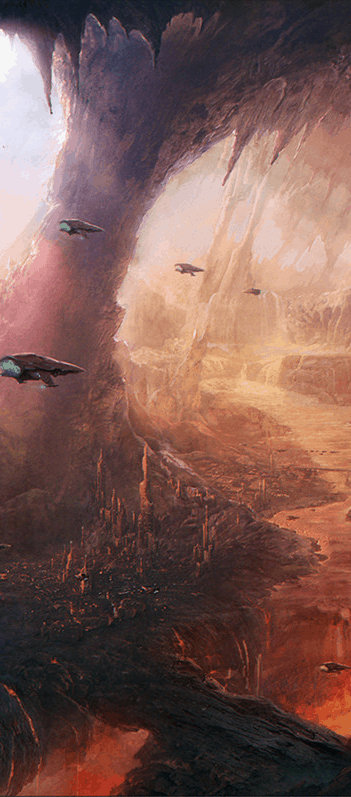
\includegraphics[width=\linewidth]{img/personnages/handicap.jpg}


\clearpage
\subsection{Atouts}

Voici le liste des Atouts disponibles dans \swr.

\subsubsection{Background}
\begin{description}[align=left]
    \item [Ambidextre]
    	\emph{[Novice, Agi d8+]}\\
        Votre héros utilise ses deux mains avec la même facilité. Il ignore le malus de -2 habituel pour la main non-directrice.

    \item [Arcane (Force)]
    	\emph{[Novice, spécial]}\\
        L’atout indispensable si votre héro doit utiliser la Force. Avec cet atout les héros est en mesure d’utiliser les \emph{Pouvoirs Innés}. Voir la section sur La~Force (p.~\pageref{sec:force}).

    \item [Brave]
    	\emph{[Novice, spécial]}\\
        Ceux qui possèdent cet Atout ont appris à maîtriser leurs peurs, à moins qu’ils ne soient tout simplement émotionnellement distants de tout. Quoi qu’il en soit, ils bénéficient d’un bonus de +2 sur les tests de terreur.

    \item [Chanceux]
    	\emph{[Novice]}\\
        Votre héros semble être béni par le destin. Il obtient un Jeton de plus au début de chaque session de jeu, ce qui lui octroie plus de chance de réussir ses actions et de survivre à d’incroyables dangers.

    \item [Très Chanceux]
    	\emph{[Novice, Chanceux]}\\
        Votre héros obtient 2 Jetons de plus au début de chaque session de jeu.

    \item [Costaud]
    	\emph{[Novice, Force et Vigueur d6+]}\\
        Votre héros est très corpulent ou tout simplement très athlétique. Dans tous les cas, sa masse lui permet de mieux résister aux dégâts. Ajoutez +1 à sa Résistance.

		En outre, votre héros est également capable de porter 4 fois sa Force en kg sans malus, au lieu de 2 fois chez les gens ordinaires.

    \item [Don des langues]
    	\emph{[Novice, Intellect d6+]}\\
        Le personnage a un don pour les langues : il commence le jeu en connaissant un nombre de langues égal à son Intellect, et peut faire un jet d’Intellect à -2 pour se faire comprendre en n’importe quel langage qu’il a côtoyé pendant au moins une semaine.

    \item [Enragé]
    	\emph{[Novice]}\\
        Dès qu’il est blessé (ou même Secoué par une attaque physique) votre héros doit réussir un jet d’Intellect sans quoi il devient Enragé. L’état Enragé inflige un malus de -2 à la Parade du personnage mais ajoute +2 à sa Résistance, à tous ses jets de Combat et de Force ainsi qu’aux dégâts causés au corps à corps.

        Le héros ignore en outre tous les malus de blessures, mais il ne peut se servir de Compétences, d’Atout, ou effectuer des man\oe{uvres} qui requièrent de la concentration comme Tir et Sarcasme. L’utilisation de la Compétence Intimidation est toutefois toujours possible. Un personnage enragé attaque sans aucune retenue. S’il obtient un résultat de 1 sur son dé de Combat (sans tenir compte du dé Joker) il touche au hasard une cible adjacente autre que le cible prévue, ami ou ennemi. En l’absence de cible adjacente le coup est juste manqué. Un personnage enragé peut calmer sa rage s’il ne fait aucune action (ni même se déplacer) pendant un round entier et s’il réussit un jet d’Intellect à -2.

    \item [Guérison rapide]
    	\emph{[Novice, Vigueur d8+]}\\
        Votre héros récupère vite de ses blessures. Il obtient un bonus de +2 à ses jets de Vigueur pour guérison naturelle.

    \item [Noble]
    	\emph{[Novice]}\\
        Les personnages de haute naissance sont avantagés par la vie mais ont aussi plus de responsabilités. Un Noble possède un statut élevé dans sa société, a droit à un traitement de faveur de la part de ses ennemis, voit son Charisme augmenté de 2 et obtient l’Atout Riche. Il obtient plusieurs Atouts pour le prix d’un mais ses responsabilités en tant qu’aristocrate équilibrent ces avantages. 

        Un Noble dispose de troupes à ses ordres, de terres, d’une demeure ancestrale et d’autres biens à gérer. Ces aspects sont à définir par le MJ et doivent inclure la charge qui pèse sur le personnage. Un Noble disposera d’une troupe de soldats, d’une forteresse. Mais cela signifiera aussi qu’il devra gouverner sa province, rendre la justice et surveiller son voisin jaloux qui convoite ses terres, complotant sans cesse contre lui.

    \item [Résistance à la Force]
    	\emph{[Novice, \^Ame d8+]}\\
        Votre héro, même s’il ne sait pas l’utiliser, est capable de résister à la Force quand elle est employée contre lui. Il obtient 2 points d’Armure contre les dégâts provoqués par des pouvoirs de la Force et bénéficie d’un bonus de +2 à ses jets pour résister aux effets de ces pouvoirs.

    \item [Grande résistance à la Force]
    	\emph{[Novice, Résistance à la Force]}\\
        Idem que ci-dessus mais l’Armure et la résistance passent à 4.

    \item [Riche]
    	\emph{[Novice]}\\
        Que votre héros soit né avec une cuillère en argent dans la bouche ou bien qu’il ait bien réussi en affaires, une chose est sûre~: il est beaucoup plus fortuné que la plupart des gens.

		Un héros Riche débute avec 3x les fonds initiaux prévus. Si le héros travaille il reçoit un salaire annuel de 150~000\crg.

    \item [Très riche]
    	\emph{[Novice, Riche ou Noble]}\\
        Votre héros est riche comme Crésus. Il débute avec 5x les fonds initiaux prévus, et, si c’est approprié, reçoit un revenu annuel de 500~000\crg. Un héros Très riche doit avoir une histoire personnelle très détaillée à valider avec le MJ. Les biens et la fortune qu’il possède impliquent autant de gestion que de lourdes responsabilités.

    \item [Séduisant]
    	\emph{[Novice, Vigueur d6+]}\\
        Votre héros a beaucoup de charme ou est très beau. Son Charisme est augmenté de 2.

    \item [Très séduisant]
    	\emph{[Novice, Séduisant]}\\
        Votre héros est d’une beauté à couper le souffle. Son Charisme est augmenté de 4.

    \item [Véloce]
    	\emph{[Novice, Agilité d6+]}\\
        Le héros se déplace très rapidement. Son Allure est augmentée de 2 et il utilise un d10 au lieu du d6 lorsqu’il court.

    \item [Vif]
    	\emph{[Novice, Agilité d8+]}\\
        Votre héros est né avec des réflexes presque surhumains. Si vous piochez un 5 ou une carte inférieure en combat, vous pouvez la défausser et en piochez une autre jusqu’à ce que vous obteniez une carte supérieure à 5. 

        Ceux qui ont les Atouts Tête froide et Sang-froid piochent d’abord toutes les cartes supplémentaires liées à ces Atouts, puis choisissent la meilleure de toutes avant d’utiliser l’Atout Vif.

    \item [Vigilant]
    	\emph{[Novice]}\\
        Peu de choses échappent à votre héros. Il est vigilant et très observateur. Il ajoute +2 à tous ses jets de Perception pour entendre, regarder ou percevoir le monde qui l’entoure.
\end{description}

\begin{paperbox}{Arcane (Force)}
    Remplace l’atout Arcanes. C’est l’atout qui représente la Force.
\end{paperbox}

\begin{paperbox}{Résistance à la Force}
    Comme son niveau supérieur Grande Résistance à la Force, cet atout remplace la résistance aux Arcanes. Il correspond comme son nom l’indique à la capacité que le héros a de résister à la Force.

    Il confère au héro 2 points d’Armure contre les dégâts provoqués par la Force et ainsi qu’un bonus de +2 aux jets pour résister aux effets de ces pouvoirs. Utiliser un pouvoir bénéfique sur le personnage n’implique pas de malus, cet atout ne se déclenche qu’à la volonté du héro.

    Pour la grande résistance, le bonus d’Armure passe à 4.
\end{paperbox}

\newpage
\subsubsection{Combat}
\begin{description}[align=left]
    \item [Arme fétiche]
    	\emph{[Novice, Combat ou Tir d10+]}\\
        Le héros ne jure que par une arme qu’il connaît par c\oe{ur} (Arbalète Laser, Bâton électrique ou même ce bon vieux blaster Bryar). Quand il se bat avec cette arme il gagne +1 à ses jets de Tir ou de Combat. Il est possible de prendre cet Atout plusieurs fois pour des armes différentes. On peut remplacer une Arme fétiche perdue mais il faut patienter deux semaines pour que revienne le bonus de l’Atout.

    \item [Arme fétiche adorée]
    	\emph{[Vétéran, Arme fétiche]}\\
        Même chose que pour Arme fétiche mais le bonus est de +2.

    \item [Arts martiaux]
    	\emph{[Novice, Combat d6+]}\\
        Ce personnage est entraîné aux techniques de combat à mains nues et n’est du coup jamais sujet à la règle sur les Défenseurs désarmés. Lors d’une attaque réussie à mains nues, il fait des dégâts de For + d4, comme s’il portait une arme légère.

    \item [Maître des arts martiaux]
    	\emph{[Vétéran, Arts martiaux, Combat d10+]}\\
        Le personnage fait des dégâts de For + d6 lors d’une attaque à mains nues.

    \item [Bagarreur]
    	\emph{[Novice, Force d8+]}\\
        Votre héros a l’habitude de cogner avec ses poings, et fort ! Quand il touche une cible avec une attaque à mains nues, il ajoute +2 aux dégâts occasionnés.

    \item [Cogneur]
    	\emph{[Aguerri, Bagarreur]}\\
        Lorsqu’un cogneur obtient une Relance lors d’une attaque à mains nues, il rajoute un d8 au lieu d’un d6 aux dégâts.

    \item [Balayage]
    	\emph{[Novice, Force d8+, Combat d8+]}\\
        Cet Atout permet au personnage d’attaquer toutes les cibles adjacentes en un seul jet de Combat avec un malus de -2. Faites un jet de dégâts pour chaque cible touchée. Les alliés du héros sont affectés par cette attaque, aussi le héros devra rester prudent quant à l’utilisation de cet Atout. Il n’est pas possible d’utiliser les Atouts Balayage et Frénésie dans le même Round.

    \item [Grand balayage]
    	\emph{[Vétéran, Balayage]}\\
        Même chose que pour Balayage mais sans le malus de -2.

    \item [Blocage]
    	\emph{[Aguerri, Combat d8+]}\\
        Les héros endurcis au corps à corps sont plus habiles à se défendre que les autres. Ils savent attaquer mais ont aussi appris à bloquer les coups ennemis. Un héros qui possède cet Atout ajoute 1 à sa Parade.

    \item [Grand blocage]
    	\emph{[Vétéran, Blocage]}\\
        Même chose que pour Blocage mais le bonus est de +2.

    \item [Combat à deux armes]
    	\emph{[Novice, Agilité d8+]}\\
        Votre héros n’est pas ambidextre mais sait se battre avec deux armes en même temps. Quand il attaque avec une arme dans chaque main il fait un jet pour chaque attaque mais il ignore le -2 pour la pénalité d’Actions multiples.

    \item [Combatif]
    	\emph{[Aguerri]}\\
        Votre héros se ressaisit vite après un coup ou une émotion forte. Il ajoute +2 à ses jets d’\^Ame pour se remettre de l’état Secoué.

    \item [Contre-attaque]
    	\emph{[Aguerri, Combat d8+]}\\
        Les combattants disposant de cet Atout sont capables de répondre instantanément aux erreurs de leurs adversaires. Une fois par round, lorsqu’un ennemi rate une attaque de corps à corps contre lui, le personnage peut faire une attaque gratuite en contre attaquant. L’attaque subit un malus de -2, et doit être une attaque normale (pas de désarmement, attaque totale ou toute autre man\oe{uvre}), et ne peut être combinée avec d’autres Atouts comme Frénésie ou Balayage. Il peut être utilisé avec la man\oe{uvre} Défense, mais pas avec Défense totale.

    \item [Grande contre-attaque]
    	\emph{[Vétéran, Contre-attaque]}\\
        Comme contre-attaque, mais sans le malus de -2.

    \item [Dégaine comme l’éclair]
    	\emph{[Novice, Agilité d8+]}\\
        Cet Atout permet au héros de dégainer une arme et d’attaquer dans le même round sans subir le malus usuel de -2. S’il doit faire un jet d’Agilité pour dégainer une arme il ajoute +2 à son jet.

    \item [Esquive]
    	\emph{[Aguerri, Agilité d8+]}\\
        L’expérience a appris à votre héros comment esquiver les mauvais coups. Grâce à cet Atout, il sait se mettre vite à couvert ou se déplacer rapidement pour éviter d’être touché. Ses ennemis ont un malus de -1 à leurs jets de Tir et de Lancer, sauf dans les cas d’une attaque surprise. Quand il tente d’échapper aux effets d’une attaque de zone il ajoute +1 à son jet d’Agilité (si la situation le permet).

    \item [Grande esquive]
    	\emph{[Vétéran, Esquive]}\\
        Même chose que pour Esquive mais les attaquants subissent -2 à leurs jets d’attaque et le héros ajoute +2 à son jet d’Agilité pour échapper aux effets d’une Attaque de zone.

    \item [Extraction]
    	\emph{[Novice, Agilité d8+]}\\
        Lorsqu’un personnage se retire d’un combat, les attaquants à son contact gagnent une attaque gratuite, une situation très risquée pour tous ! Fort heureusement, votre héros a l’habitude de ce genre de retraites.

		En réussissant un jet d’Agilité lors d’une retraite, un adversaire de votre choix ne disposera pas d’attaque gratuite.

    \item [Grande extraction]
    	\emph{[Novice, Extraction]}\\
        Comme Extraction, mais en cas de Relance sur le jet d’Agilité, aucun adversaire au contact du personnage ne bénéficiera d’une attaque gratuite.

    \item [Frappe éclair]
    	\emph{[Novice, Agilité d8+]}\\
        Une fois par round votre héros obtient une attaque de Combat gratuite contre un seul ennemi venant au contact, à condition de ne pas être Secoué. Ceci interrompt automatiquement l’action de l’adversaire et ne coûte pas la sienne au héros s’il est en attente ou n’a pas encore fait d’action dans le round.

    \item [Frappe foudroyante]
    	\emph{[Héroïque, Frappe éclair]}\\
        Même chose que pour Frappe éclair, mais le héros obtient une attaque de Combat supplémentaire contre chacun des ennemis venant au contact.

    \item [Frénésie]
    	\emph{[Aguerri, Combat d10+]}\\
        Frénésie en combat de mêlée permet de faire pleuvoir des coups rapides sur ses adversaires au détriment de la précision. Le héros obtient une attaque de Combat en plus par round avec un malus de -2 à tous ses jets d’attaques. Cette attaque doit être appliquée en même temps qu’une autre attaque de Combat mais peut cibler deux ennemis différents adjacents au héros (les Joker lancent deux dés de Combat et un dé Joker). Le malus de -2 s’applique sur toutes les attaques. 

        Un personnage muni de deux armes ne fait toutefois qu’une attaque en plus.

    \item [Frénésie suprême]
    	\emph{[Vétéran, Frénésie]}\\
        Même chose que pour Frénésie mais sans le malus de -2.

    \item [Improvisation martiale]
    	\emph{[Aguerri, Intellect d6+]}\\
        Les héros se trouvent parfois avec du matériel non destiné au combat. Votre héros est capable d’utiliser ce genre d’objets en tant qu’armes improvisées. Il ne subit pas le malus de -1 normalement appliqué aux jets de Combat et à la Parade lorsqu’il s’en sert dans un combat au corps à corps.

    \item [Increvable]
    	\emph{[Joker, Novice, Âme d8+]}\\
        Votre héros a plus de vies qu’un camion rempli de chats. Lorsqu’il doit lancer les dés quand il passe dans un \'Etat critique ou sur la Table des blessures il ignore les malus dus aux blessures. Seul les jets de Vigueur sur ces tables sont concernés : il subit toujours les malus pour blessures pour les autres jets de Traits.

    \item [Trompe-la-mort]
    	\emph{[Joker, Novice, Âme d8+]}\\
        Votre héros est plus dur à tuer que Raspoutine lui-même. Si jamais il est tué, lancez un dé. Sur un résultat impair il est vraiment mort. Par contre, un résultat pair signifie que d’une façon ou d’une autre il échappe à la mort et n’est que dans un \'Etat critique. Il peut être fait prisonnier, être dépouillé ou simplement laissé pour mort, mais d’une manière ou d’une autre, il est toujours en vie.

    \item [Instinct de tueur]
    	\emph{[Héroïque]}\\
        Votre héros déteste perdre. Dans un cas d’égalité sur un jet opposé, il gagne. En outre, s’il fait un 1 sur son dé lors d’un jet Opposé, il peut relancer le dé (mais doit garder le second résultat, même s’il s’agit d’un nouveau 1).

    \item [Nerfs d’acier]
        \emph{[Novice, Vigueur d8]}\\
        Votre héros a appris à combattre en ignorant la douleur. Il ignore 1 point de malus dus aux Blessures.

    \item [Nerfs d’acier trempés]
    	\emph{[Novice, Nerfs d’Acier]}\\
        Même chose que pour Nerfs d’acier, mais 2 points de malus pour blessures sont ignorés.

    \item [Panache]
    	\emph{[Novice, \^Ame d8+]}\\
        Quand ce héros met tout son c\oe{ur} dans une tache, ça se voit ! Quand il dépense un Jeton sur un jet de Trait (y compris un jet d’encaissement), il ajoute +2 au résultat final.

    \item [Poigne ferme]
    	\emph{[Novice, Agilité d8+]}\\
        Votre héros ignore le malus de -2 de Plateforme instable pour tirer depuis un véhicule ou sur une monture en mouvement.

    \item [Rock’n’rolla]
    	\emph{[Aguerri, Tir d8+]}\\
        Les tireurs expérimentés ont appris à maîtriser le recul provoqué par les armes automatiques. Si un héros muni de cet Atout ne se déplace pas, il ignore le malus de -2 du à l’effet de recul de ce type d’armes.

    \item [Sans pitié]
    	\emph{[Aguerri]}\\
        Le personnage peut utiliser un Jeton pour relancer un jet de dégâts, y compris pour une attaque de zone.

    \item [Tête froide]
    	\emph{[Aguerri, Intellect d8+]}\\
        Celui qui garde son calme quand les autres courent aux abris est un adversaire redoutable. Cet Atout permet au héros de piocher une carte en plus pour l’Initiative. Il fait son action sur la meilleure des cartes.

    \item [Sang-froid]
    	\emph{[Aguerri, Tête froide]}\\
        Même chose que pour Tête froide, mais le héros pioche 2 cartes supplémentaires.

    \item [Tireur d’élite]
    	\emph{[Aguerri]}\\
        Le héros vise juste et bien. S’il ne bouge pas durant le round il tire comme s’il avait pris la man\oe{uvre} Viser. Cet Atout ne fonctionne pas avec une arme ayant une Cadence de Tir supérieure à 1.
		
		Cet Atout s’applique aux Compétences Tir et Lancer.

    \item [Tueur de géant]
    	\emph{[Vétéran]}\\
        En général plus c’est grand plus c’est dur à vaincre. Mais votre héros sait trouver les points faibles des créatures de grande taille. Votre héros ajoute 1d6 à ses dégâts lorsqu’il attaque des créatures d’au moins trois tailles supérieure à la sienne.
\end{description}

\subsubsection{Combat au Sabre Laser}
\begin{description}[align=left]
    \item [Shii-Cho\label{itm:shii-cho}]
        \emph{[Padawan/Apprenti]}\\
        Votre héros a été formé à la première forme de maniement du Sabre Laser (p. \pageref{sec:sabre-laser}). Il ne subit plus le malus de -2 lors de son utilisation et ne risque plus de se blesser lors d’un échec critique.

    \item [Soresu]
        \emph{[Shii-Cho]}\\
        Forme de la Résistance, c’est un technique non-agressive, basée sur la défense, qui permet au Jedi de contrer les tirs de blaster.\\
        Lorsqu’il se sert de son Sabre Laser, le héros ajoute +1 à sa parade et ses adversaires ont un malus de -1 à leurs jets de Tir et de Lancer.

    \item [Maître Soresu]
        \emph{[Soresu]}\\
        Même chose que Soresu mais le héros ajoute +2 à sa parade et ses adversaires ont un malus de -2 à leurs jets de Tir et de Lancer.

    \item [Djem So]
        \emph{[Soresu]}\\
        La Forme de la Persévérance est une forme agressive et puissante qui permet de retourner les tirs de blasters vers l’envoyeur. \\
        Une fois par round, lorsqu’un ennemi rate un tir énergétique contre lui, le personnage peut faire une attaque gratuite en contre attaquant. L’attaque subit un malus de -2, et doit être effectuée avec la compétence \emph{Maîtrise de la Force}, elle ne peut être combinée avec d’autres Atouts. Les dégâts infligés par l’attaque sont ceux de l’arme énergétique déviée. Cette Atout ne peut être utilisé durant la man\oe{uvre} Défence Totale.

    \item [Maître Djem So]
        \emph{[Djem So]}\\
        Même chose que Djem So mais sans le malus -2 sur l’attaque.

    \item [Jar’Kai]
        \emph{[Shii-Cho]}\\
        C'est la Forme qui permet au Jedi de manier deux sabres laser.

        Le héros ajoute +1 à ses jets de Combat contre un adversaire muni d’une arme et sans bouclier. En outre, les bonus d’Attaque à plusieurs de ses ennemis sont diminués de 1 car le héros utilise avec brio ses deux armes pour parer leurs coups.

        Cet atout vaut aussi pour les Sabres double.

\end{description}

\newpage
\subsubsection{Commandement}
Les Atouts de commandement permettent aux héros d’employer aux mieux leurs alliés et leurs troupes lors des batailles, en les rendant plus efficaces, plus sûrs ou plus résistants. Ces Atouts s’appliquent sur les alliés sous votre commandement dans un rayon de 5 cases (l’aura de commandement). 

Si différents héros ont des Atouts de Commandement identiques ils n’en cumulent pas les effets. Si deux héros possèdent l’Atout Commandement, leurs troupes n’en bénéficient pas deux fois mais elles peuvent dans tous les cas profiter des effets d’Atouts de commandement différents comme Inspiration et Ferveur par exemple, même si ces Atouts proviennent de deux commandants différents.

\begin{description}[align=left]
    \item [Commandement]
    	\emph{[Novice, Intellect d6+]}\\
        Votre héros sait donner des ordres clairs et se faire obéir. Cela rend vos alliés plus disposés à se battre malgré les coups. Vos alliés ajoutent +1 à leurs jets d’\^Ame pour se remettre d’un état Secoué.

    \item [Ferveur]
    	\emph{[Vétéran, Âme d8+, Commandement]}\\
        Une seule phrase prononcée par un grand chef produit parfois des résultats stupéfiants. Un chef doté de cet Atout stimule la ferveur combative de ses Alliés en criant un slogan, une devise ou simplement des mots d’encouragement. Vos Alliés ajoutent +1 aux dégâts de leurs jets de Combat.

    \item [Grande aura de commandement]
    	\emph{[Novice, Commandement]}\\
        Une voix forte, des ordres précis, un charisme naturel, ou tout simplement un entraînement hors du commun, quoi qu’il en soit, votre héros est un officier qui sait commander sur le champ de bataille. Son aura de commandement est effective jusqu’à 10 cases au lieu de 5.

    \item [Inspiration]
    	\emph{[Aguerri, Commandement]}\\
        Les chefs célèbres et expérimentés sur le champ de bataille motivent les soldats autour d’eux. Ils ajoutent +2 à leurs jets d’\^Ame pour se remettre d’un état Secoué (incluant déjà le bonus de +1 de l’Atout Commandement). Cela augmente les chances des Alliés de se remettre de leurs blessures légères ou d’un moral en berne qui en temps normal leur aurait fait abandonner le combat.

    \item [Leader naturel]
    	\emph{[Novice, Âme d8+, Commandement]}\\
        Un lien spécial unit votre héros et ses alliés. Ce lien lui permet d’utiliser ses Jetons pour n’importe quel allié sous ses ordres.

    \item [Meneur d’hommes]
    	\emph{[Vétéran, Commandement]}\\
        Votre héros est fait pour commander. Les mots justes lui viennent naturellement. Tout dans son équipe se passe de manière huilée. Les alliés sous son commandement utilisent un d10 comme Joker au lieu de d6 lorsqu’ils font des jets de groupe.

    \item [Serrez les rangs !]
    	\emph{[Aguerri, Intellect d8+, Commandement]}\\
        Cet Atout renforce la détermination des Alliés aux ordres du héros. Les troupes ajoutent 1 à leur Résistance.

    \item [Tacticien]
    	\emph{[Aguerri, Commandement, Joker, Intellect d8+, Connaissance (Batailles) d6+]}\\
        Le héros a une compréhension naturelle des tactiques militaires impliquant des petites unités, et peut fréquemment tirer parti d’une situation évoluant rapidement.

        Au début d’un combat, avant que les cartes d’action aient été distribuées, le héros fait un jet de Connaissance (Batailles). Pour chaque succès et Relance, il reçoit une carte d’action. Ces cartes sont conservée séparément des cartes d’actions normales et ne sont pas mélangées jusqu’à la fin du combat (ni même dans le cas d’un joker). Au début d’un round, le héros peut donner une ou plusieurs cartes à ses alliés, qu’ils soient Extras ou Jokers, qui la considère ainsi alors comme leur carte du round.

        Un seul personnage par camp peut utiliser cet Atout durant une rencontre.

\end{description}

\newpage
\subsubsection{Pouvoir}

\begin{description}[align=left]
    \item [Drain de l’\^ame]
        \emph{[Aguerri, Arcanes (Force), Connaissance (Force) d10+]}\\
        Quand votre héros a besoin d’urgence de Points de pouvoir il utilise cet Atout pour drainer cette énergie du fond de son âme. 

        Avant d’utiliser cette dangereuse faculté, le héros décide d’abord du nombre de Points de pouvoir qu’il veut drainer. Il fait alors un jet d’\^Ame avec comme malus le nombre de points choisi (c’est une Action gratuite). Si le résultat de son dé d’\^Ame est de 1 ou moins, le héros encaisse une blessure et perd aussitôt conscience durant 1d6 heures. Sur un échec il subit une Blessure. Avec un succès ou mieux le héros obtient les Points de pouvoir désirés et s’en sert aussitôt pour activer un pouvoir (ces points ne se conservent pas).

    \item [Nouveau pouvoir]
        \emph{[Novice, Arcanes]}\\
        Cet Atout, qui peut être pris plusieurs fois, permet au héros d’apprendre un nouveau pouvoir. Il en choisit un parmi tous ceux disponibles. Attention certains pouvoir ont des pré-requis. Voir la section sur La Force (p. \pageref{sec:force}).

    \item [Points de pouvoir]
        \emph{[Novice, Arcanes]}\\
        Padawan, Jedi ou autre utilisateur de la Force ont toujours besoin de plus de pouvoir. Cet Atout leur donne 5 Points de pouvoir en plus.

        Cet Atout peut être pris plusieurs fois mais seulement une fois par Rang.

    \item [Source de pouvoir]
        \emph{[Aguerri, Âme d6+, Arcanes]}\\
        Cet Atout permet au héros de récupérer 1 Point de Pouvoir toutes les 30 minutes au lieu de toutes les heures.

    \item [Grande source de pouvoir]
        \emph{[Vétéran, Source de pouvoir]}\\
        Le héros récupère 1 Point de Pouvoir toutes les 15 minutes.

    \item [Padawan]
        \emph{[Aguerri, \^Ame d8+, Arcane (Force)]}\\
        La sensibilité de votre héro à la force a été remarqué et l’ordre Jedi l’accepte comme padawan sous la tutelle d’un Maître. 

        Votre héro peut alors apprendre, avec l’aide de son maître, à utiliser les \emph{Pouvoirs \'Elémentaires}. Voir la section sur La Force (p. \pageref{sec:force}). Le malus d’utilisation de Sabre Laser passe à \textbf{-2} (cf. Sabre Laser (p. \pageref{sec:sabre-laser}).

    \item [Apprenti Sith]
        \emph{[Aguerri, \^Ame d8+, Arcane (Force)]}\\
        La haine et la ranc\oe{ur} de votre héro ont donné des idées à un Seigneur Sith qui décide de le prendre comme apprenti.

        Votre héro peut alors apprendre, avec l’aide de son maître, à utiliser les \emph{Pouvoirs \'Elémentaires}. Voir la section sur La Force~\ref{sec:force} (p. \pageref{sec:force}). Le malus d’utilisation de Sabre Laser passe à \textbf{-2} (cf. Sabre Laser (p. \pageref{sec:sabre-laser}).

    \item [Maître Jedi]
        \emph{[Vétéran, \^Ame d10+, Padawan, Maîtrise de la Force d10+]}\\
        Après sa formation de Padawan votre héro pourra devenir un Maître Jedi. Cela implique qu’il prête serment à l’Ordre et surtout qu’il respecte ce serment.

        Le Maître Jedi a accès, en plus des pouvoirs disponibles pour les Padawan, à tout les \emph{Pouvoirs Universels} et \emph{Pouvoirs du coté Lumineux}. Voir la section sur La Force (p. \pageref{sec:force}). Le malus d’utilisation de Sabre Laser disparaît (cf. Sabre Laser (p. \pageref{sec:sabre-laser}).

        Il bénéficie en plus du soutien de l’ordre en terme de renseignement et de ressources, il obtient un bonus de +2 sur ses jets de Réseau qui ont trait au coté Clair.

    \item [Seigneur Sith]
        \emph{[Vétéran, \^Ame d10+, Apprenti Sith, Maîtrise de la Force d10+]}\\
        Votre héro, après avoir prêté serment à son Maître, devient à son tour un seigneur Sith. Il accède alors à tous les \emph{Pouvoirs Universels} et les \emph{Pouvoirs du coté Obscur}. Voir la section sur La Force (p. \pageref{sec:force}). Le malus d’utilisation de Sabre Laser disparaît (cf. Sabre Laser (p. \pageref{sec:sabre-laser}).

        Il bénéficie en plus des conseils de son maître, il obtient un bonus de +2 sur ses jets de Réseau qui ont trait au coté Obscur.

    \item [Adepte Sauvage]
        \emph{[Aguerri, \^Ame d8+, Arcane (Force), Maîtrise de la Force d10+]}\\
        En tant qu’adepte, votre héro a accès à tout les \emph{Pouvoirs \'Elémentaires} et \emph{Pouvoirs Universels} mais n’ayant été au bout de sa formation, il ne pourra jamais maîtriser les Pouvoirs des différents coté de la Force. De plus, les Adeptes ne bénéficient d’aucun soutien.

        Cet atout est effaçable moyennant une progression.
        
\end{description}

\begin{paperbox}{Adeptes Sauvages}
A l’origine les Adeptes Sauvages se sont formé dans le but de purger l’Ordre Jedi, coupable à leur yeux d’avoir abandonné face aux Sith et d’être devenu faible, incapable de ralentir la montée du Second Empire Sith. Il est essentiellement composé de Déchiqueteurs, descendants corrompus d’utilisateurs de la Force. Les Adeptes étant sensible à la force, sont capable d’utiliser ses Pouvoirs. Mais n’ayant jamais réellement penché pour une doctrine, ils ne parviennent pas à utiliser les Pouvoir spécifiques au coté clair ou obscur.

Sont aussi considéré comme Adepte Sauvage les individus solitaires n’ayant pour une raison ou une autre pas souhaité ou pas peu terminer leur formation (Ex: Luke qui interrompt sa formation pour sauver ses amis). 

Cet atout remplace l’atout Professionnel \emph{Adepte}.
\end{paperbox}

\newpage
\subsubsection{Professionnels}

\begin{description}[align=left]

    \item [Acrobate]
        \emph{[Novice, Agilité d8+, Force d6+]}\\
        Ceux qui ont un entraînement dans la pratique des acrobaties peuvent choisir cet Atout. Il ajoute +2 à tous leurs jets d’Agilité pour accomplir une man\oe{uvre} acrobatique (Ruses incluses) et ajoute 1 à leur Parade quand ils ne subissent pas de malus d’Encombrement.

    \item [As du volant]
        \emph{[Novice, Agilité d8+]}\\
        Les As sont ces virtuoses plus à l’aise derrière un volant ou des leviers de commandes que sur leurs deux jambes.

        Un As du volant ajoute +2 à tous ses jets de Conduite, de Navigation et de Pilotage. Il peut aussi dépenser des Jetons pour faire des jets d’encaissement pour tout véhicule qu’il contrôle. Pour cela, il doit réussir son jet de Conduite, de Navigation ou de Pilotage à -2 (annulant ainsi le bonus de +2 de l’Atout). Chaque succès et Relance annule une Blessure et toute Dégradation critique qui en aurait découlé.

    \item [Assassin]
        \emph{[Novice, Agilité d8+, Combat d6+, Discrétion d8+, Escalade d6+]}\\
        Les assassins sont des tueurs entraînés à tuer avec une précision mortelle, du moins s’ils sont capable d’approcher suffisamment leur proie. Ils ont un bonus de +2 à leurs dégâts lorsqu’ils frappent une cible ne les ayant pas vu venir (même avec une attaque à distance).

    \item [Bidouilleur]
        \emph{[Novice, Intellect d10+, Réparation d8+, 2 Connaissances scientifiques à d6+]}\\
        Le Bidouilleur ajoute +2 à tous ses jets de Réparer. En outre, s’il obtient une Relance sur son jet il divise par deux le temps nécessaire pour la réparation. Si une réparation indique qu’une Relance permet de réparer l’objet en moitié moins de temps que d’ordinaire, un Bidouilleur fera alors le travail dans le quart de temps requis avec un Relance.

    \item [Débrouillard]
        \emph{[Novice, Intellect d6+, Réparation d6+, Perception d8+]}\\
        Quand il a besoin d’un outil indisponible, ce personnage sait comment improviser. Il ne subit aucun malus sur ses jets de Traits dus au manque d’outils dans la plupart des situations. En plus, avec quelques objets, outillage ou machines simples il arrive à bricoler un appareil sommaire qui lui permet de se tirer de pièges mortels ou de créer des objets bizarre quand ces derniers font défaut. La portée de cet Atout reste soumise à l’appréciation du meneur de jeu mais la créativité devrait être récompensée particulièrement lors de situations difficiles où il n’y a pas trop de solutions.

    \item [\'Erudit]
        \emph{[Novice, 2 Connaissances à d8+]}\\
        Les \'Erudits sont des professeurs émérites, des étudiants appliqués et des amateurs enthousiastes qui passent leur temps à étudier certaines matières. Ils deviennent experts dans ces matières et peuvent répondre à la plupart des questions sur leur domaine d’expertise. Choisissez deux Compétences de Connaissances à d8 ou plus. Chaque fois que vous les utilisez, ajoutez +2 à vos jets de dé. Ceux qui étudient l’histoire militaire ont ainsi un avantage quand ils dirigent des troupes dans une grande bataille. Un bonus de +2 à un jet de Connaissances (Batailles) peut faire la différence entre une victoire foudroyante et une débâcle.

    \item [Forestier]
        \emph{[Novice, Âme d6+, Survie d8+, Pistage d8+]}\\
        Un Forestier est un ranger, un éclaireur ou un chasseur, plus à l’aise dans les étendues sauvages qu’en milieu urbain. Excellent pisteur et éclaireur il sait aussi trouver tout ce qu’il faut pour survivre en milieu sauvage. 

        Il ajoute +2 à ses jets de Pistage, Survie et Discrétion. Le bonus pour la Discrétion ne s’applique qu’en milieu sauvage.

    \item [Investigateur]
        \emph{[Novice, Intellect d8+, Recherche d8+, Réseaux d8+]}\\
        Un Investigateur a consacré du temps à investiguer sur d’anciennes légendes, à enquêter dans les rues et à résoudre d’infâmes mystères. Certains sont détectives privés, d’autres des professeurs d’université découvrant des « Secrets Que l’Homme ne Doit Pas Savoir ». Un Investigateur ajoute +2 à tous ses jets de Réseaux, de Recherche et aux les jets de Perception lorsqu’il cherche des indices.

    \item [Touche-à-Tout]
        \emph{[Novice, Intellect d10+]}\\
        Votre héros possède un talent pour toucher à de nombreux domaines. Autodidacte ou juste doté d’une intuition et d’un sens de l’observation phénoménal, ce personnage arrive toujours à savoir comment ça marche.

        Chaque fois qu’il doit faire un jet par défaut sur une compétence dérivant d’Intellect, il lance un d4 au lieu du d4-2 ordinaire.

    \item [Voleur]
        \emph{[Novice, Agilité d8+, Escalade d6+, Piratage d6+, Discrétion d8+]}\\
        Un voleur est spécialiste en mystification, en forfaiture et en acrobaties. Il pratique avec adresse les arts malhonnêtes et est apprécié là où les pièges doivent être détectés, les murs escaladés et les serrures déverrouillés. Le voleur ajoute +2 à tous ses jets de Escalade, Piratage et Discrétion. Le bonus à la Discrétion ne s’applique qu’en milieu urbain et non en milieu naturel.
\end{description}

\newpage
\subsubsection{Sociaux}

\begin{description}[align=left]

    \item [Charismatique]
        \emph{[Novice, Âme d8+]}\\
        Votre héros sait s’y prendre avec les gens même avec ceux qui s’opposent à lui ou à ses efforts. Son Charisme est augmenté de 2.

    \item [Contacts]
        \emph{[Novice]}\\
        Que ce soit l’alliance rebelle, l’empire, la fédération du commerce, votre héros connaît quelqu’un qui en fait partie et est disposé à l’aider à l’occasion (une fois par session de jeu). Cet Atout peut être pris plusieurs fois, s’appliquant chaque fois à une organisation différente. Le MJ doit également s’assurer que l’organisation reste limitée à une entité. Pour utiliser son contact, le héros doit d’abord le joindre. Il fait un jet de Réseaux. Un échec signifie que le contact est injoignable (hors de portée, occupé, etc\ldots).

        Une fois mis en relation le héros fait un jet de Persuasion. Libre au MJ de modifier ce jet et tout résultat selon les circonstances. Un échec signifie que le contact du héros ne peut rien pour cette fois ci ou bien qu’il n’est pas persuadé que son aide soit nécessaire. Avec un succès, le contact peut fournir des informations mais ne prendra pas de risques pour aider le personnage.

        Avec une Relance, le contact fournit des informations essentielles mais n’ira pas jusqu’à trahir ses sources. Deux Relances et plus signifient que votre héros peut compter sur un sérieux coup de main. Le contact prendra de vrais risques pour lui. Si un soutien financier est nécessaire, le contact lui donne un peu plus que nécessaire. S’il a besoin d’une aide musclée, le contact lui fournira soit un expert soit cinq hommes de main en fonction de l’organisation pour laquelle il travaille.

    \item [Lien mutuel]
        \emph{[Joker, Novice, Âme d8+]}\\
        Cet Atout représente le lien qui unit des compagnons comme un groupe d’aventuriers. Qu’ils s’entendent bien ou pas, ils ont tissé des rapports étroits au cours de leurs nombreuses aventures épiques.

        Un héros doté de cet Atout peut donner ses Jetons à tout autre Joker avec lequel il peut communiquer. Cela représente son soutien verbal ou moral. Le joueur doit dire ce que fait ou dit son personnage pour donner ce soutien, comme un discours ou un petit geste d’encouragement.

    \item [Volonté de Fer]
        \emph{[Novice, Intimidation d6+, Sarcasmes d6+]}\\
        Un héros au caractère trempé utilise sa voix, son regard d’acier ou son esprit vif pour déstabiliser ses adversaires. Un personnage doté d’une Volonté de fer ajoute +2 à ses jets d’Intimidation et de Sarcasme et à ses jets d’\^Ame et d’Intellect quand il résiste à une Épreuve de volonté.
\end{description}

\newpage
\subsubsection{\'Etranges}

Il s’agit là d’atouts spéciaux n’ayant pas un grand rapport avec Star Wars mais ils ont un coté fun dont il serait dommage de se priver.

\begin{description}[align=left]
    \item [Courage liquide]
        \emph{[Novice, Agilité d8+]}\\
        Votre héros assimile l’alcool de manière bien inhabituelle. Le round après avoir consommé une boisson alcoolisée (au moins un quart de litre d’alcool fort), la Vigueur du personnage passe au dé supérieur (et la Résistance augmente mécaniquement de 1). Il peut également ignorer le malus d’un niveau de Blessure (cumulable avec d’autres capacités ou Atouts similaires).

        Il subit aussi un malus de -2 à tous les jets basés sur l’Agilité ou l’Intellect tant qu’il continue à boire, et 1d6 heures après.

    \item [Maître des bêtes]
        \emph{[Novice]}\\
        Peut être est-ce l’odeur ou peut être que votre héro use de la Force inconsciemment mais les animaux l’aiment et ne l’attaqueront pas, à moins qu’il ne les attaque en premier lieu où qu’ils ne soient enragés pour une raison quelconque. Il dispose d’un tel magnétisme animal qu’une bête s’est attachée à lui (un chien, un loup, voire même un Wampa). Au MJ d’approuver l’animal. Si l’animal meurt une autre la remplace au bout de 2d6 jours si la situation le permet.

    \item [Recycleur]
        \emph{[Novice, Chanceux]}\\
        Une fois par session, le héros peur se rappeler soudainement qu’il a en sa possession un objet utile. Cet objet doit pouvoir tenir en poche ou dans un sac, et le meneur de jeu a toujours le dernier mot quant à ce qui peut être trouvé ou non.

    \item [Sixième sens]
        \emph{[Novice]}\\
        Il l’ignore mais la Force est avec votre héros. Chaque fois qu’il va être victime d’une attaque surprise, d’une embuscade ou d’un autre vilain tour du style, il peut faire un jet de Perception à -2 juste avant que cela se produise. En cas de succès, il sait qu’il va que quelque chose va se produire et il s’y prépare. Il sera donc En attente au premier round de combat.

        En cas d’échec, le héros utilise les règles de surprise normales si nécessaire.
\end{description}

\newpage
\subsubsection{Légendaire}

Les Atouts qui suivent sont à part car rares sont les campagnes atteignant ce niveau.

\begin{description}[align=left]
    \item [Acolyte]
        \emph{[Joker, Légendaire]}\\
        Un héros qui passe son temps à vaincre les forces du mal devient un modèle pour d’autres. Parmi ceux-là, il y en a un qui désire suivre le héros dans ses aventures épiques. Le héros obtient un Acolyte de Rang Novice. C’est un Joker qui gagne aussi de l’expérience et dont les Compétences complètent ou imitent celles de son héros.

        De manière générale, le joueur contrôle son Acolyte comme il le fait pour ses alliés. Il peut arriver de temps en temps que cet Acolyte devienne une source d’ennuis (en se faisant capturer, en se jetant dans la gueule du loup sans prévenir, etc\ldots). Le joueur doit être préparé à ce que son Atout se transforme de temps à autre en Handicap.

        Si l’Acolyte meurt, il n’est pas remplacé sauf si l’Atout est de nouveau pris.

    \item [Endurci]
        \emph{[Légendaire]}\\
        Votre héros est un vétéran confirmé. Augmentez de +1 sa Résistance.

    \item [Coriace]
        \emph{[Légendaire, Endurci]}\\
        Augmentez encore la Résistance de votre héros de +1.

    \item [Maître d’Armes]
        \emph{[Légendaire, Combat d12+]}\\
        Augmentez de +1 la Parade de votre héros.

    \item [Maître d’Armes Légendaire]
        \emph{[Légendaire, Maître d’Armes]}\\
        Augmentez encore de +1 la Parade de votre héros.

    \item [Professionnel]
        \label{sec:atout-professionnel}
        \emph{[Légendaire, d12+ dans le Trait choisi]}\\
        Votre héros est devenu chevronné dans un Trait particulier. Ce trait passe à d12+1. Cet Atout peut-être pris plusieurs fois mais ne peut s’appliquer deux fois au même Trait.

    \item [Expert]
        \label{sec:atout-expert}
        \emph{[Légendaire, Professionnel dans le Trait choisi]}\\
        Comme l’Atout Professionnel, mais le Trait passe à d12+2.

    \item [Maître]
        \emph{[Joker, Légendaire, Expert dans le Trait choisit.]}\\
        Le dé Joker du héros devient un d10 quand il fait un jet sous le Trait choisi. L’Atout peut-être choisi plusieurs fois mais ne peut s’appliquer deux fois au même Trait.

    \item [Suivants]
        \emph{[Joker, Légendaire]}\\
        Les héros sont souvent entourés de soldats dévoués, de joyeux compagnons ou autres volontaires qui les suivent dans leurs aventures. Chaque fois que cet Atout est choisi, 5 suivants rejoignent votre héros. Cet Atout peut être pris plusieurs fois (pour remplacer les pertes subies au combat par exemple). 

        Les suivants doivent pouvoir se nourrir et gagner leur vie. Ils prennent en général leur part des trésors, de butin et des récompenses de votre héros. Ils sont dévoués et risquent souvent leur vie pour lui. Ils n’iront toutefois pas jusqu’au sacrifice de leur vie, sauf dans des cas exceptionnels ou dans le cas de Suivants accompagnant votre héros depuis longtemps. 

        C’est le MJ qui définit les Traits et statistiques des Suivants, mais en général, l’archétype soldat est utilisé. Les Suivants débutent avec un équipement standard. C’est au héros d’acheter tout équipement supplémentaire.

\end{description}


\subsubsection{Jokers}

Les Atouts ne fonctionnent que quand votre héros pioche un Joker lors de la phase d’Initiative en combat. Les effets de ces Atouts s’ajoutent aux effets habituels d’un Joker.

\begin{description}[align=left]
    \item [Afflux de pouvoir]
        \emph{[Joker, Aguerri, Arcane (Force) d10+]}\\
        Lorsque votre personnage pioche un Joker lors de la phase d’Initiative, il regagne aussitôt 2d6 Points de pouvoir (sans toutefois pouvoir dépasser sa limite habituelle).

    \item [Dans le mille !]
        \emph{[Joker, Aguerri, Tir ou Lancer d10+]}\\
        Le héros double le total de ses dégâts s’il réussit une attaque de Tir ou de Lancer dans ce round.

    \item [Coup puissant]
        \emph{[Joker, Aguerri, Combat d10+]}\\
        Le héros double le total de ses dégâts s’il réussit une attaque de Combat dans ce round.

\end{description}

\newpage
\clearpage
\subsection{Création d'un personnage}

\subsubsection{Race}
Choisissez la race de votre personnage parmi celles proposées.

\subsubsection{Traits}
\begin{rebelist}
	\item Votre héros débute avec un d4 dans chaque Attribut et dispose de 5 points avec lesquels il peut les augmenter. Augmenter un Attribut d’un type de 	dé coûte 1 point.
	\item Vous avez 15 points pour vos Compétences.
	\item Chaque type de dé investi dans une Compétence coûte 1 point jusqu’à égaler le dé de l’Attribut dont dépend la Compétence. Au-delà, le coût est de 	2 points.
	\item Le Charisme est égal au total des bonus ou des malus donnés par les Atouts ou les Handicaps.
	\item L’Allure est de 6 cases.
	\item La Parade est égale à 2 plus la moitié de la Compétence Combat.
	\item La Résistance est égale à 2 plus la moitié de Vigueur. Vous pouvez y ajouter le bonus de l’armure portée sur le torse pour accélérer le calcul en 	cours de partie mais ce bonus ne compte pas pour les autres parties du corps.
\end{rebelist}

\subsubsection{Atouts \& Handicaps}
Vous gagnez des points supplémentaires en prenant un Handicap Majeur (2 points) et jusqu’à deux Handicaps Mineurs (1 point chacun).

Pour 2 points vous pouvez :
\begin{rebelist}
	\item Augmenter un Attribut d’un type de dé.
	\item Choisir un Atout.
\end{rebelist}

Pour 1 point vous pouvez :
\begin{rebelist}
	\item Augmenter une Compétence d’un type de dé.
	\item Doubler vos fonds initiaux.
\end{rebelist}

\subsubsection{Équipement}
Débutez avec 500\crg.

\subsubsection{Histoire personnelle}
Rajoutez les détails concernant le personnage qui vous semblent importants.

\subsection{Progression}
Le rang détermine la puissance approximative de votre héros. Le nombre de points d’XP que vous avez gagné détermine le rang selon le tableau suivant : 

\begin{itemtable}[ l l ]
	\textbf{XP}		& \textbf{Rang} \\
	00-19 			& Novice \\
   	20-39 			& Aguerri \\
   	40-59 			& Vétéran \\
   	60-79 			& Héroïque \\
   	80+				& Légendaire
\end{itemtable}

Tout les 5XP votre héros bénéficie d’une progression. Lors d’une progression il peut :
\begin{rebelist}
	\item Choisir un nouvel Atout.
	\item Augmenter une Compétence dont la valeur est égale ou supérieure au Trait associé.
	\item Augmenter deux Compétences dont les valeurs sont inférieures aux Traits associés.
	\item Prendre une nouvelle Compétence à d4.
	\item Augmenter un Attribut d’un type de dé. Vous ne pouvez choisir cette option qu’une fois par Rang ou lors d’une progression sur deux après avoir atteint le rang Légendaire. Il n’est pas possible de progresser au-delà de d12 dans un Trait par le biais d’une Progression, mais vous pouvez consulter les Atouts Professionnel et Expert (p.~\pageref{sec:atout-professionnel}).
\end{rebelist}

\subsection{Fiche de personnage}
Enfin, sur la page suivante la fiche de personnage. Comme tout le reste de \swr, elle est fournie avec les sources en SVG et est complètement modifiable.\\

\cite{swr-character-sheet-src}.

\clearpage

\begin{tikzpicture}[overlay, anchor=north]
    \node at (9,2) {\includegraphics[height=\paperheight]{img/swr-fiche-perso.pdf}};
\end{tikzpicture}


\clearpage 

